\documentclass[10pt,letterpaper]{article}
\usepackage[top=0.85in,left=2.75in,footskip=0.75in]{geometry}

% amsmath and amssymb packages, useful for mathematical formulas and symbols
\usepackage{amsmath,amssymb}

% Use adjustwidth environment to exceed column width (see example table in text)
\usepackage{changepage}

% Use Unicode characters when possible
\usepackage[utf8x]{inputenc}

% textcomp package and marvosym package for additional characters
\usepackage{textcomp,marvosym}

% cite package, to clean up citations in the main text. Do not remove.
\usepackage{cite}

% Use nameref to cite supporting information files (see Supporting Information section for more info)
\usepackage{nameref,hyperref}

% line numbers
\usepackage[right]{lineno}

% ligatures disabled
\usepackage{microtype}
\DisableLigatures[f]{encoding = *, family = * }

% color can be used to apply background shading to table cells only
\usepackage[table]{xcolor}

% array package and thick rules for tables
\usepackage{array}

% create "+" rule type for thick vertical lines
\newcolumntype{+}{!{\vrule width 2pt}}

% create \thickcline for thick horizontal lines of variable length
\newlength\savedwidth
\newcommand\thickcline[1]{%
  \noalign{\global\savedwidth\arrayrulewidth\global\arrayrulewidth 2pt}%
  \cline{#1}%
  \noalign{\vskip\arrayrulewidth}%
  \noalign{\global\arrayrulewidth\savedwidth}%
}

% \thickhline command for thick horizontal lines that span the table
\newcommand\thickhline{\noalign{\global\savedwidth\arrayrulewidth\global\arrayrulewidth 2pt}%
\hline
\noalign{\global\arrayrulewidth\savedwidth}}

\usepackage{float}

% Remove comment for double spacing
\usepackage{setspace} 
\doublespacing

% Text layout
\raggedright
\setlength{\parindent}{0.5cm}
\textwidth 5.25in 
\textheight 8.75in

% Bold the 'Figure #' in the caption and separate it from the title/caption with a period
% Captions will be left justified
\usepackage[aboveskip=1pt,labelfont=bf,labelsep=period,justification=raggedright,singlelinecheck=off]{caption}
\renewcommand{\figurename}{Fig}

% Use the PLoS provided BiBTeX style
% \bibliographystyle{plos2015}

% Remove brackets from numbering in List of References
\makeatletter
\renewcommand{\@biblabel}[1]{\quad#1.}
\makeatother

% Header and Footer with logo
\usepackage{lastpage,fancyhdr,graphicx}
\usepackage{epstopdf}
%\pagestyle{myheadings}
\pagestyle{fancy}
\fancyhf{}
%\setlength{\headheight}{27.023pt}
%\lhead{\includegraphics[width=2.0in]{PLOS-submission.eps}}
\rfoot{\thepage/\pageref{LastPage}}
\renewcommand{\headrulewidth}{0pt}
\renewcommand{\footrule}{\hrule height 2pt \vspace{2mm}}
\fancyheadoffset[L]{2.25in}
\fancyfootoffset[L]{2.25in}
\lfoot{\today}

%% Include all macros below

\newcommand{\lorem}{{\bf LOREM}}
\newcommand{\ipsum}{{\bf IPSUM}}

\usepackage[english]{babel}
\usepackage{natbib}
\usepackage{multirow}
\usepackage{wrapfig}
% \usepackage[nomarkers,figuresonly]{endfloat}
\usepackage[caption=false]{subfig}

% for editing
\usepackage[normalem]{ulem}

\newcommand\Mycite[1]{%
  \citeauthor{#1}~[\citeyear{#1}]}



\begin{document}
\vspace*{0.2in}

\begin{flushleft}
{\Large
\textbf\newline{Automatic interpretation of cod otoliths using deep learning}
}
\newline


Endre Moen\textsuperscript{1*},
Rune Vabø\textsuperscript{1},
Come Denechaud\textsuperscript{1},
Ketil Malde\textsuperscript{1,2},
\\
\bigskip
\textbf{1} Institute of Marine Research, Bergen, Norway
\\
\textbf{2} Department of Informatics, University of Bergen, Norway
\\
\bigskip
* endre.moen@hi.no

\end{flushleft}
% Please keep the abstract below 300 words

\linenumbers

\section*{Abstract}

The age of individual cod (Gadus morhua) is determined by manually examining the layered structure of otoliths, a calcium carbonate structure of the inner ear. Image-based methods have been tried to age otoliths with varying results, but recent developments in automatic image analysis techniques are promising. The objective of this paper is to
investigate the accuracy in aging broken otolith images on state-of-the-art convolutional neural networks.


\section*{Introduction}

Information on fish age constitutes one of the most important biological variables, which is used
in the investigations of life history (e.g. growth, sexual maturation) and population dynamics
\Mycite{campana2001accuracy}

\section*{Method and materials}

\subsection*{Data Collection}

We sampled a data set of  5150 cod otolith images, which has been collected 
on different cruises and read by otolith experts. The images are taken during
cruises in the period 2012-2018 conducted by Institute of Marine Research (IMR).
There are six images with three light exposures and one rotation.
The expert readers has varied during this time period as has the configuration
for photographing the otoliths. 

\begin{figure}[h!]
  \caption{Otolith from 2016, read age: 6. With light exposure: medium, low, high, 
  then rotated 180 degrees and three new images}
  \centering
  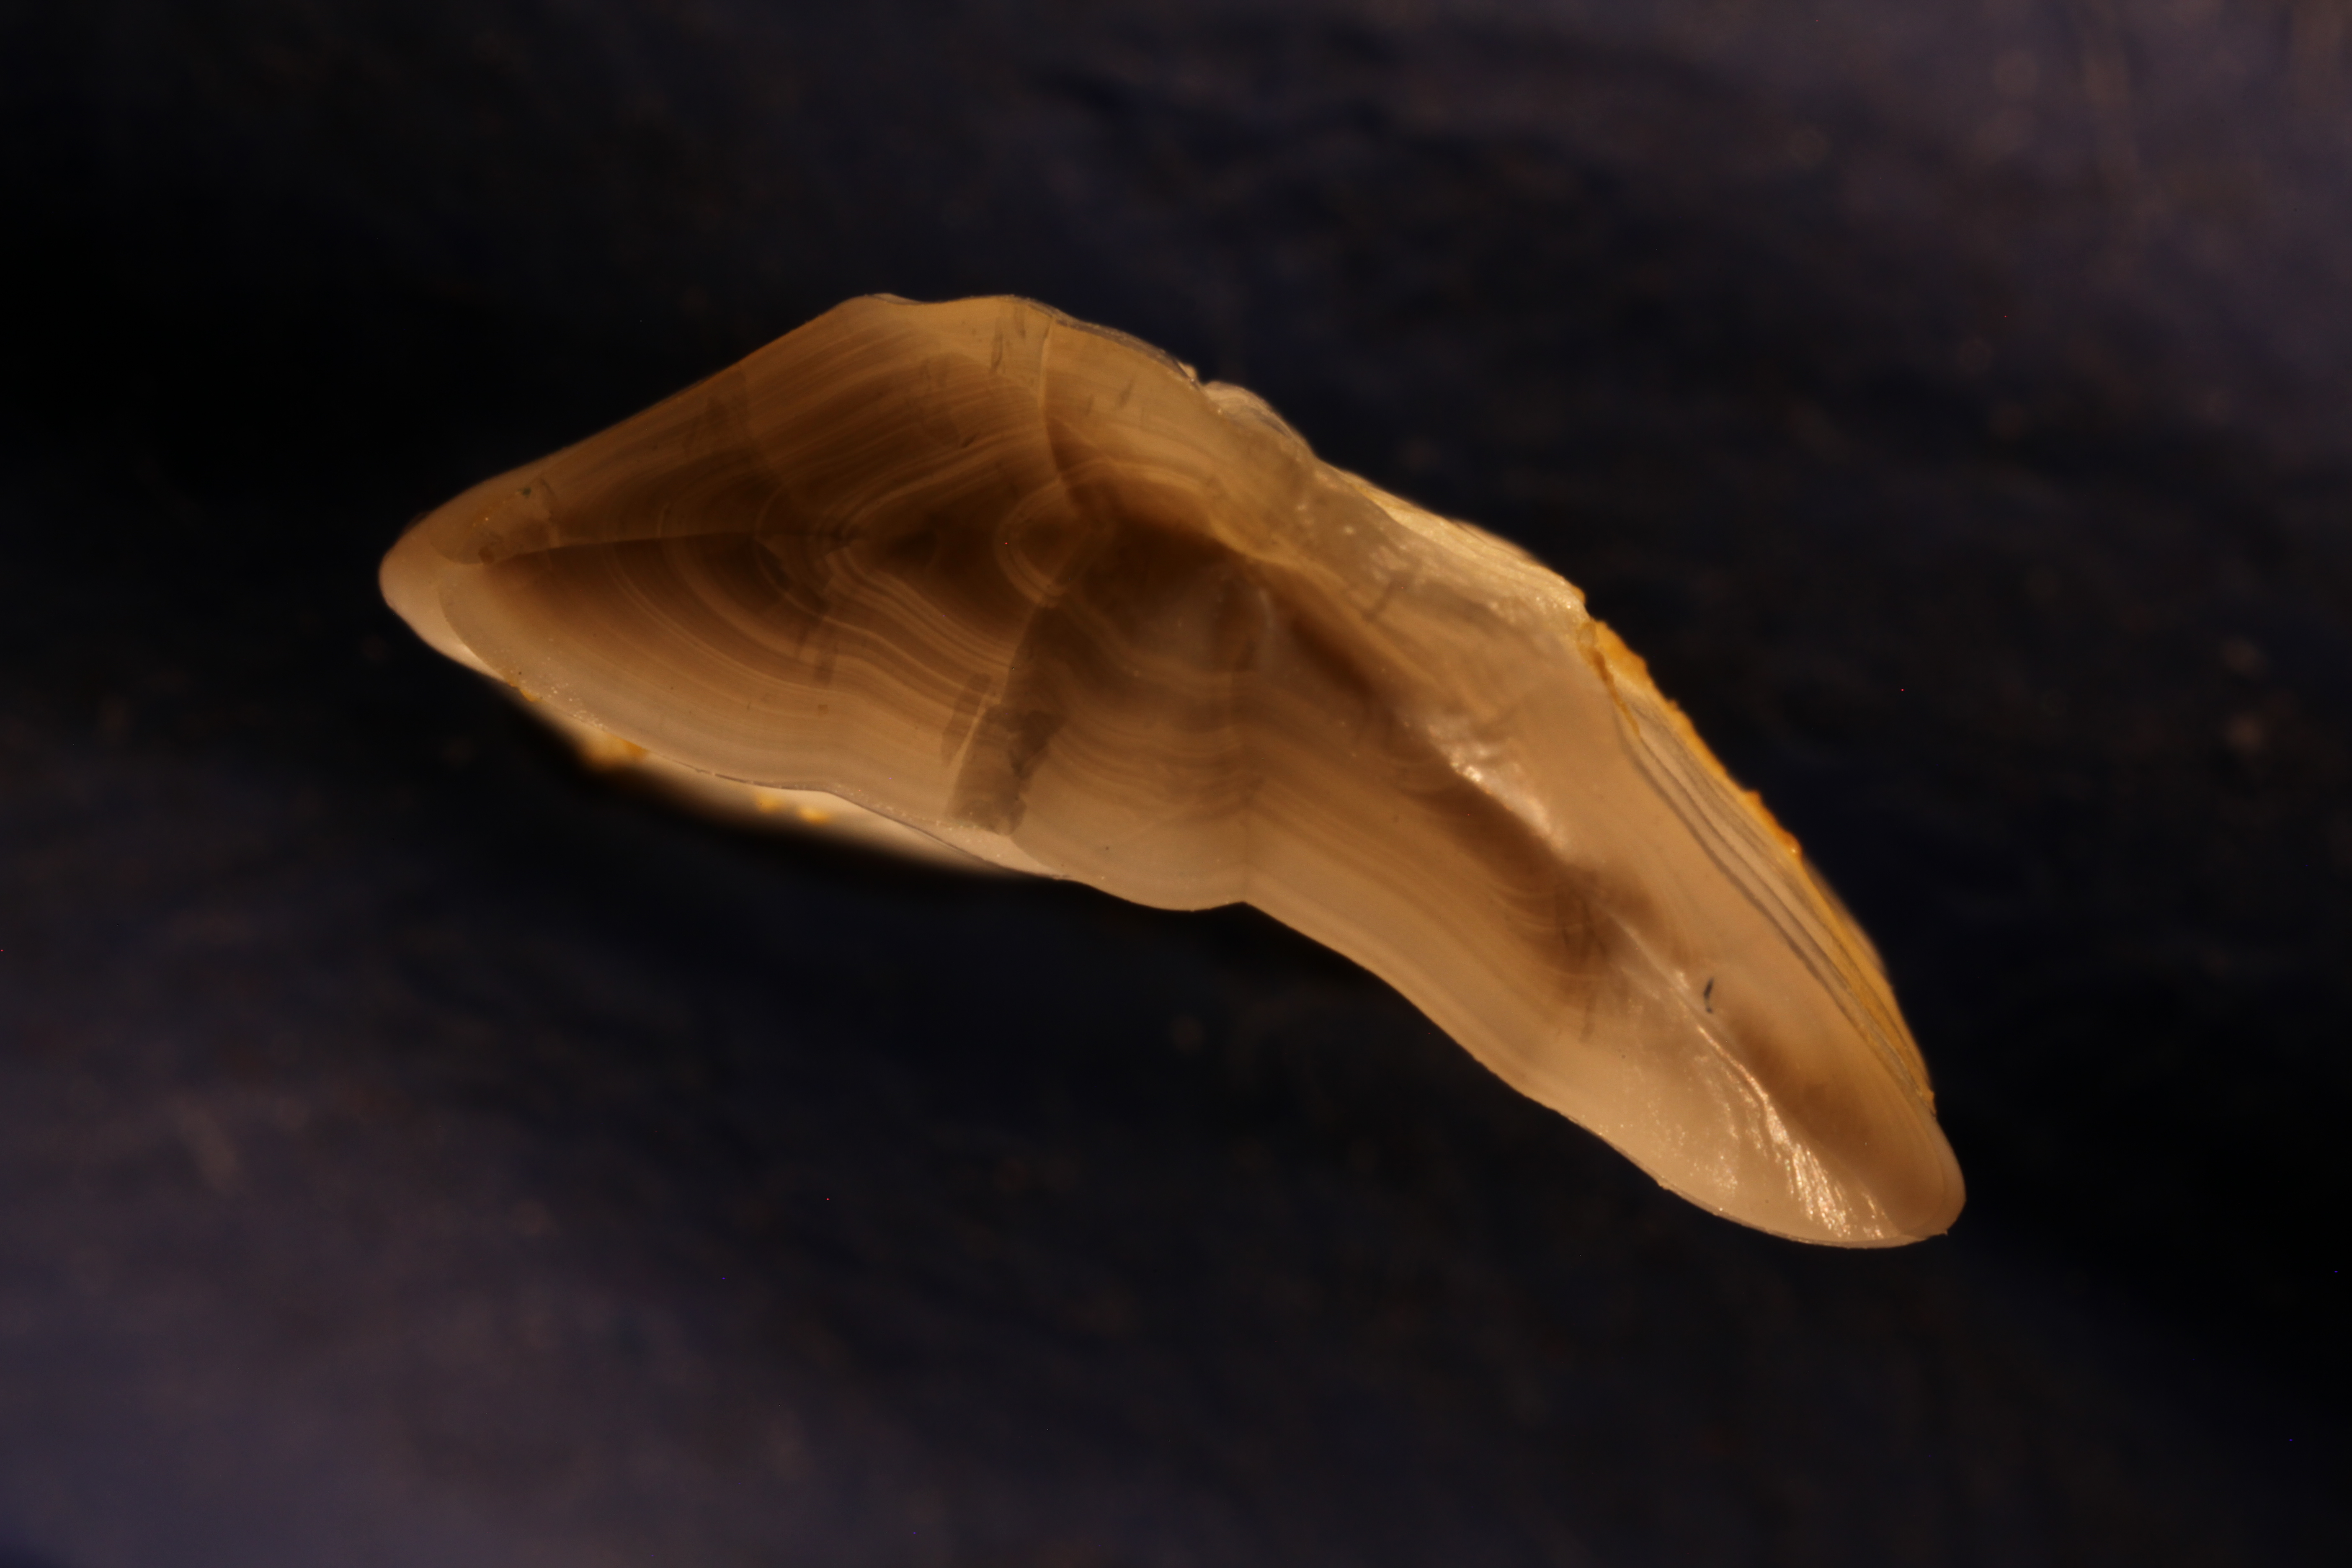
\includegraphics[scale=0.015]{otolith/IMG_0457_2016_70021.JPG}
  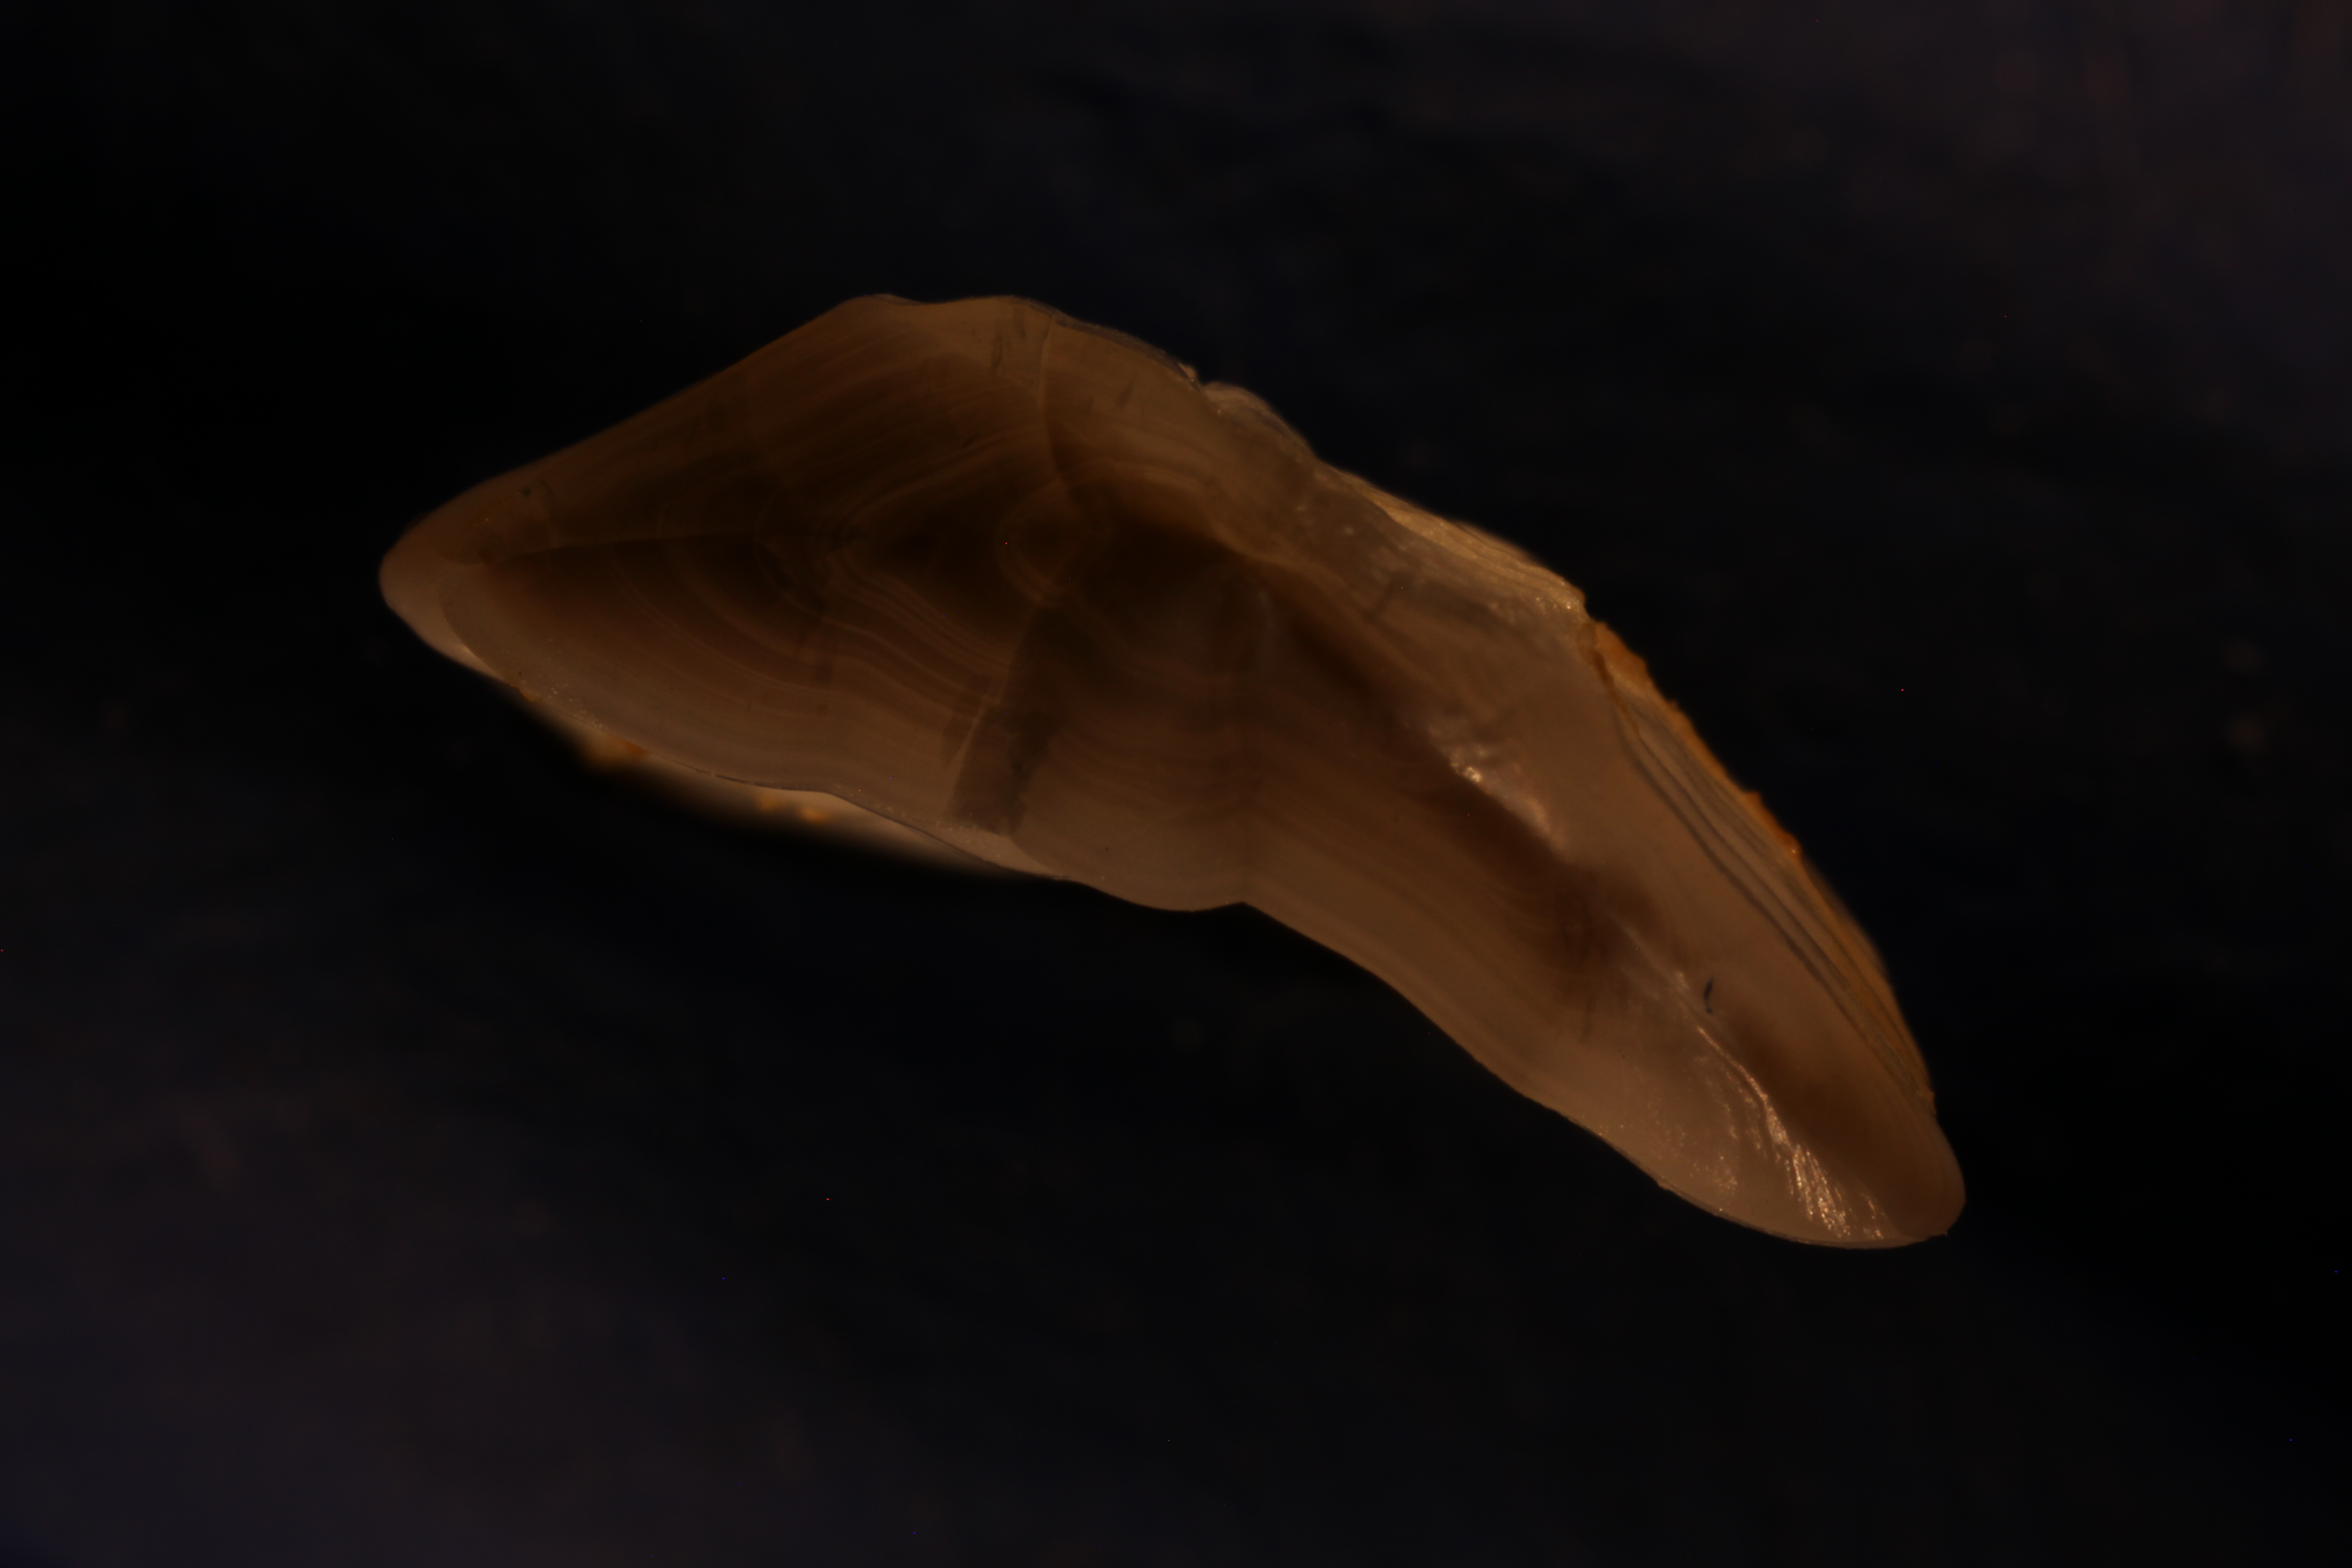
\includegraphics[scale=0.015]{otolith/IMG_0458_2016_70021.JPG}
  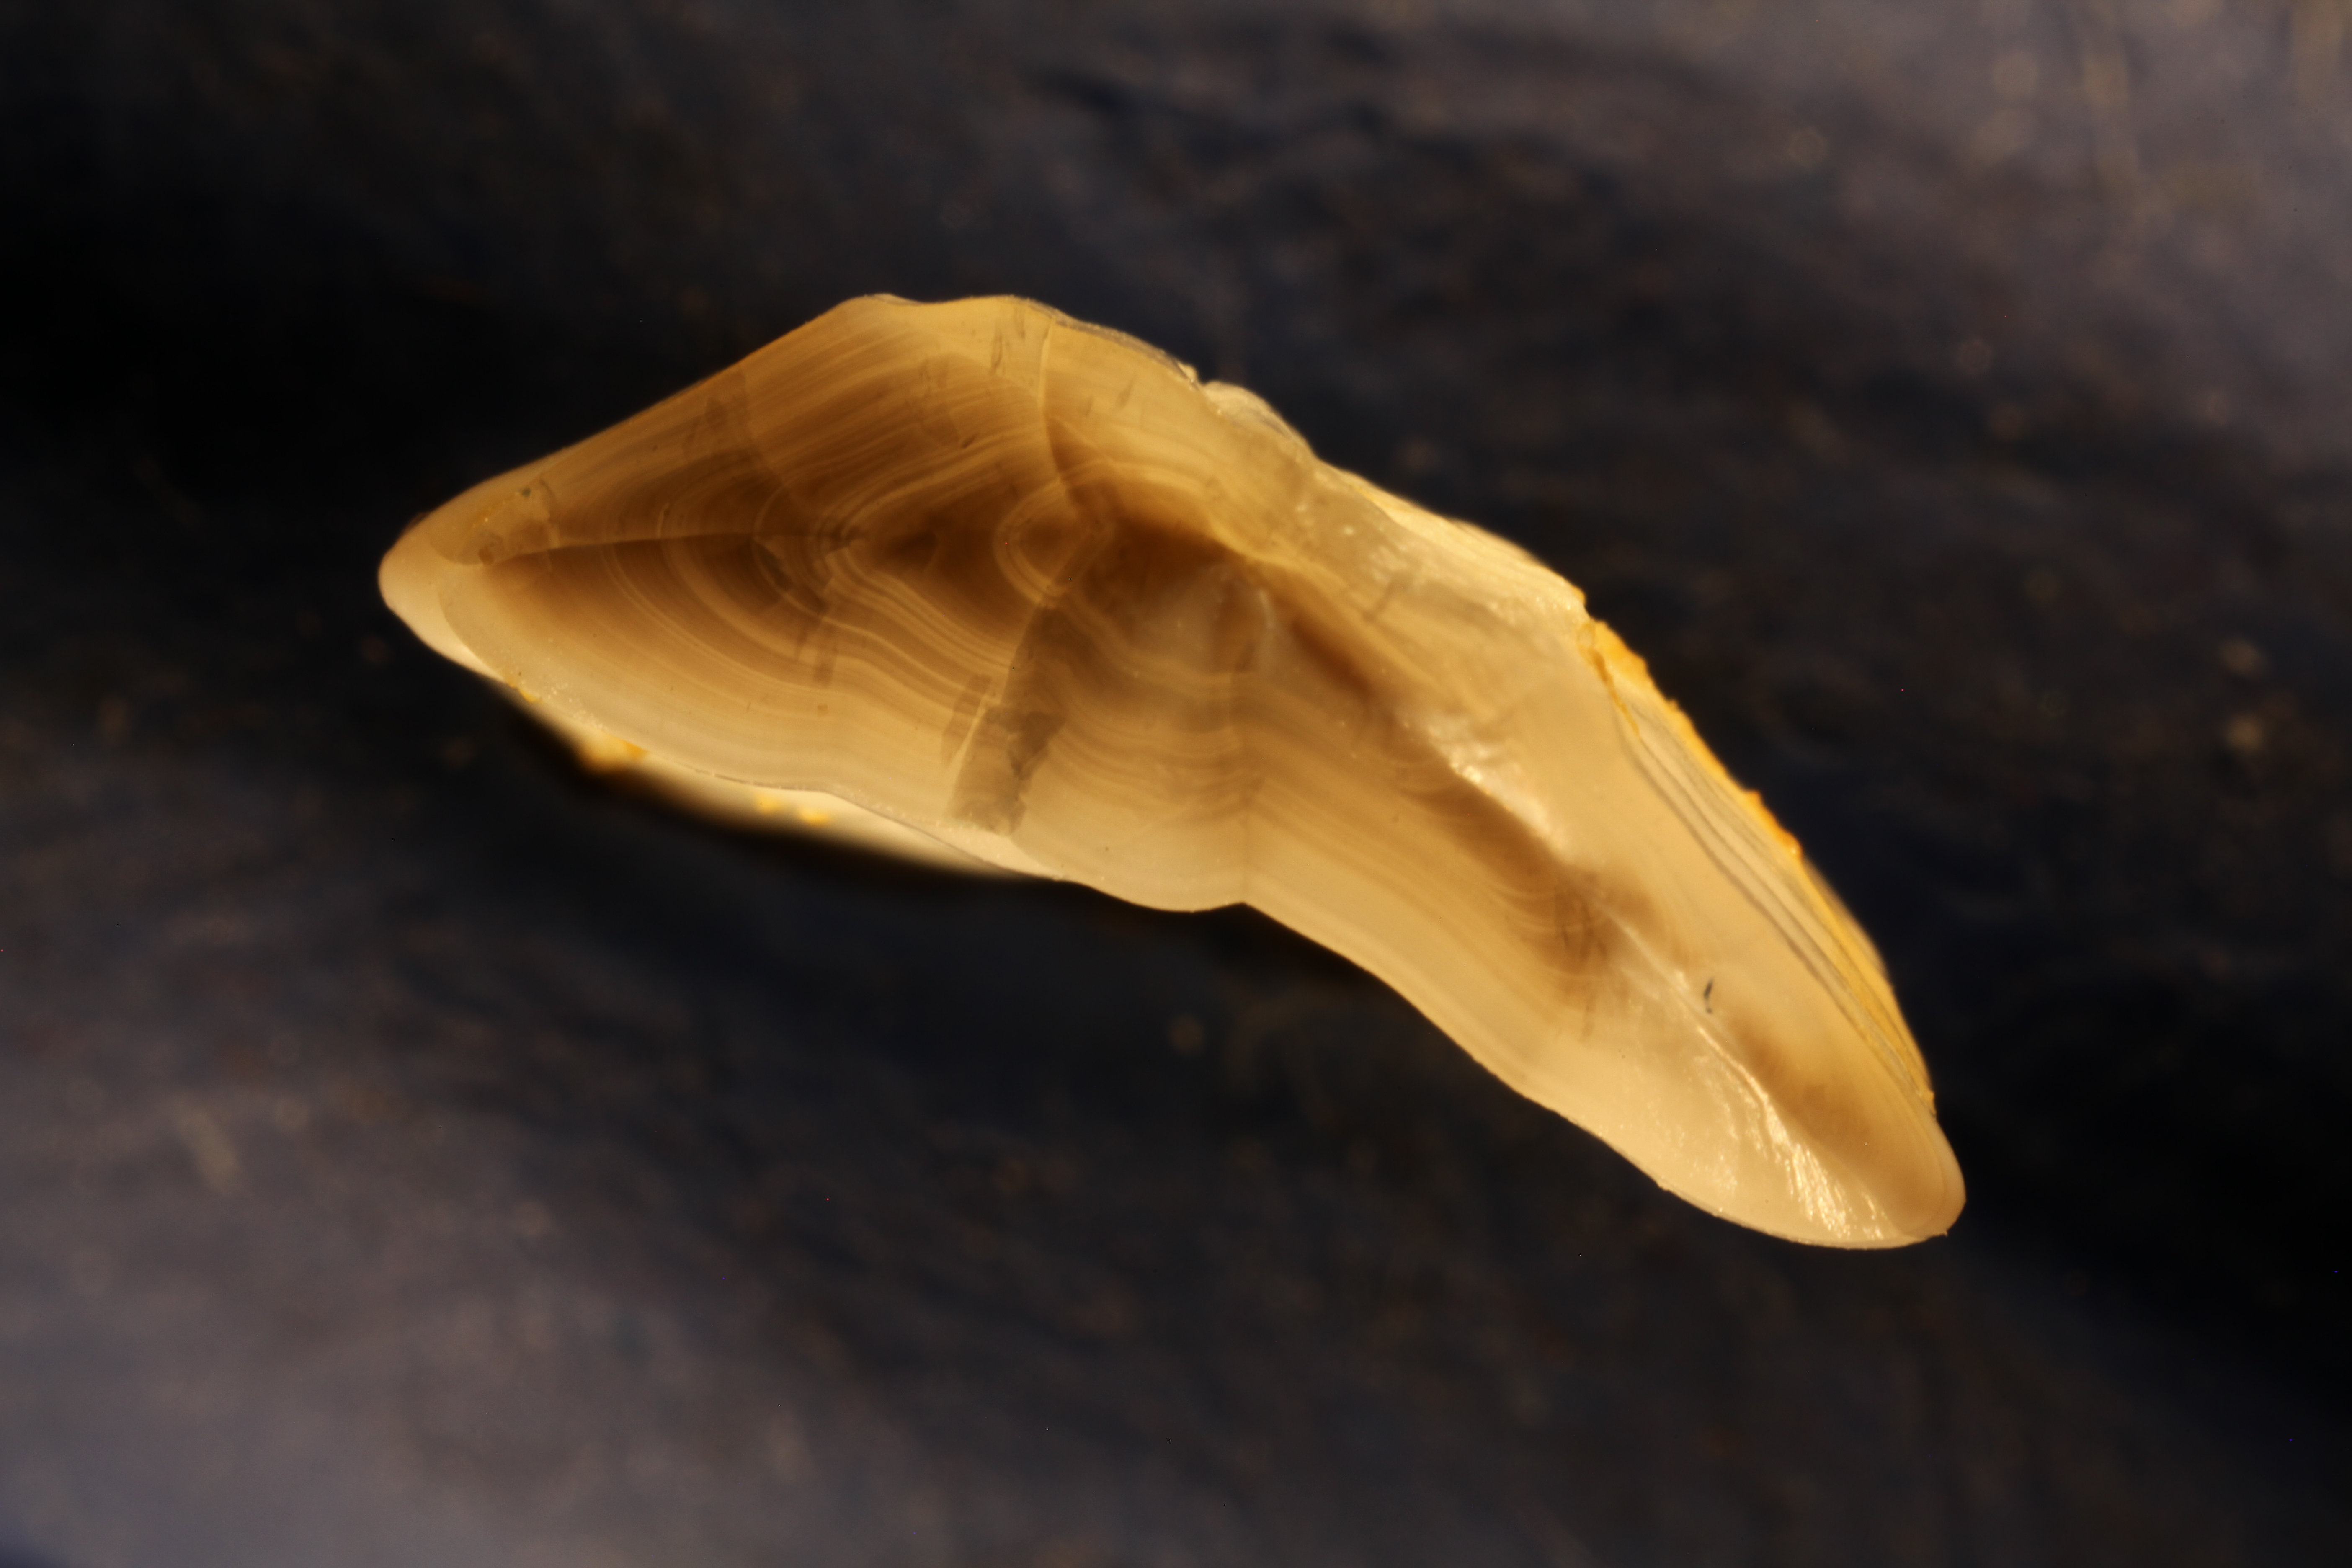
\includegraphics[scale=0.015]{otolith/IMG_0459_2016_70021.JPG} 

  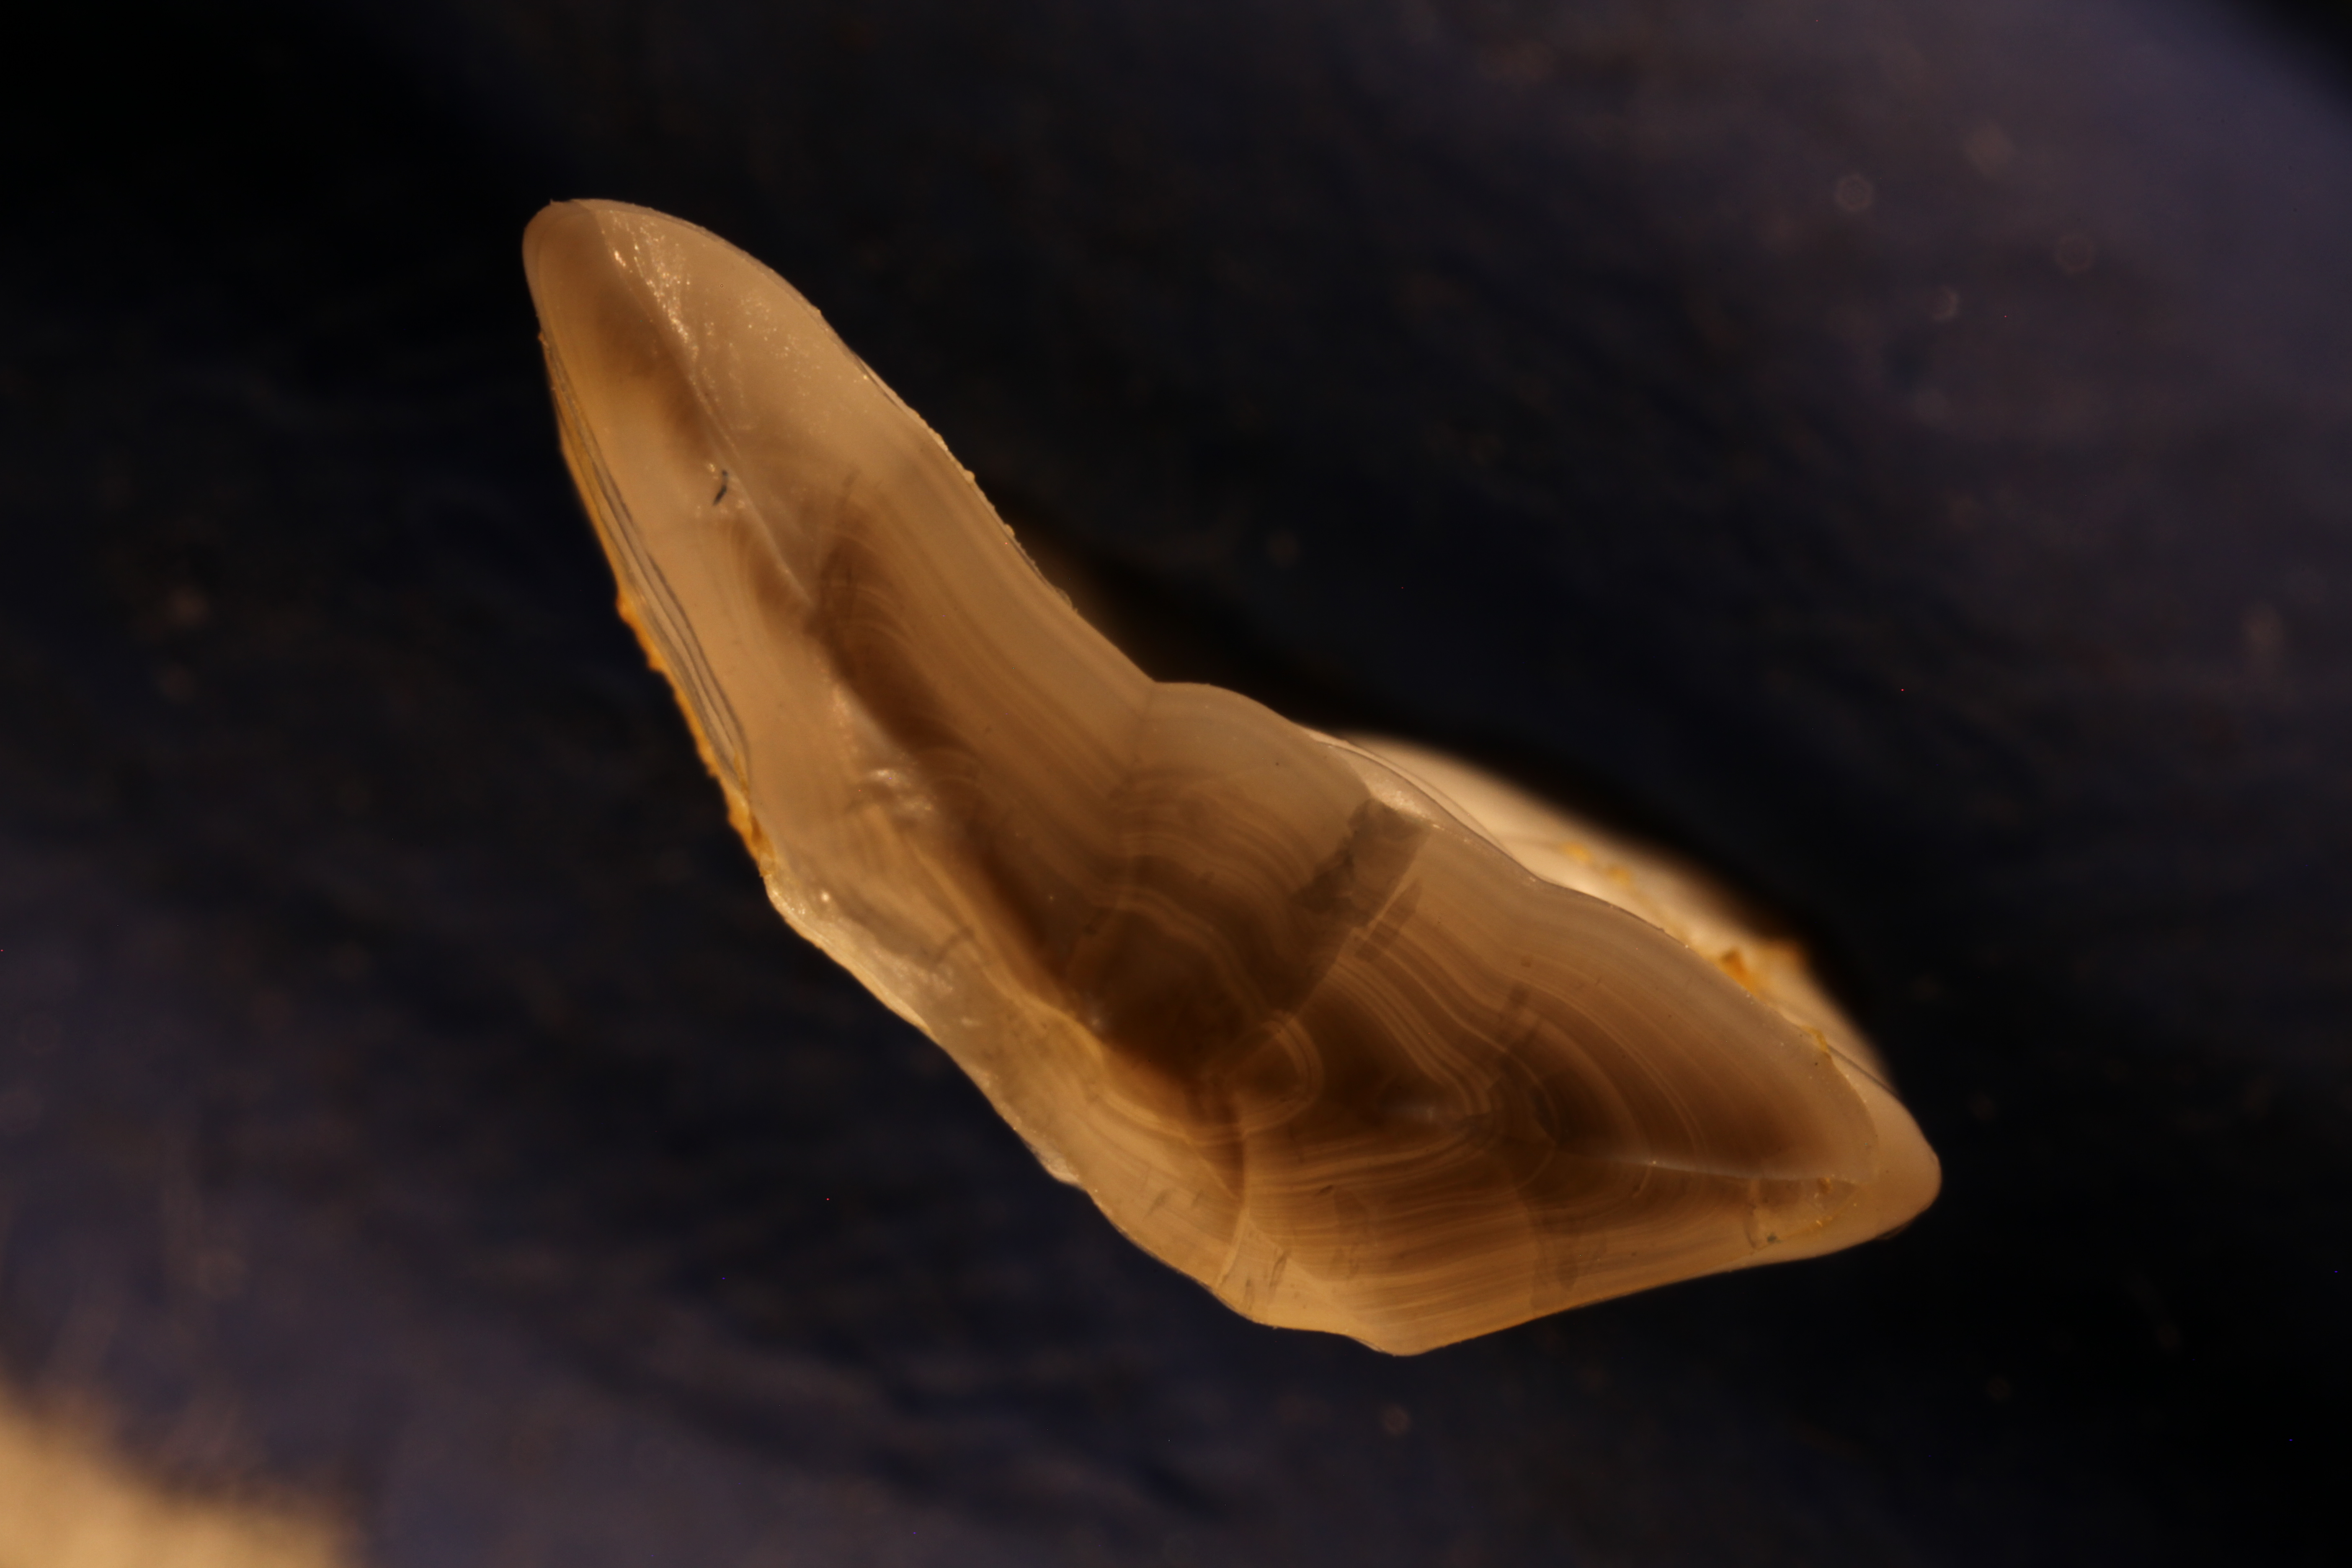
\includegraphics[scale=0.015]{otolith/IMG_0460_2016_70021.JPG}
  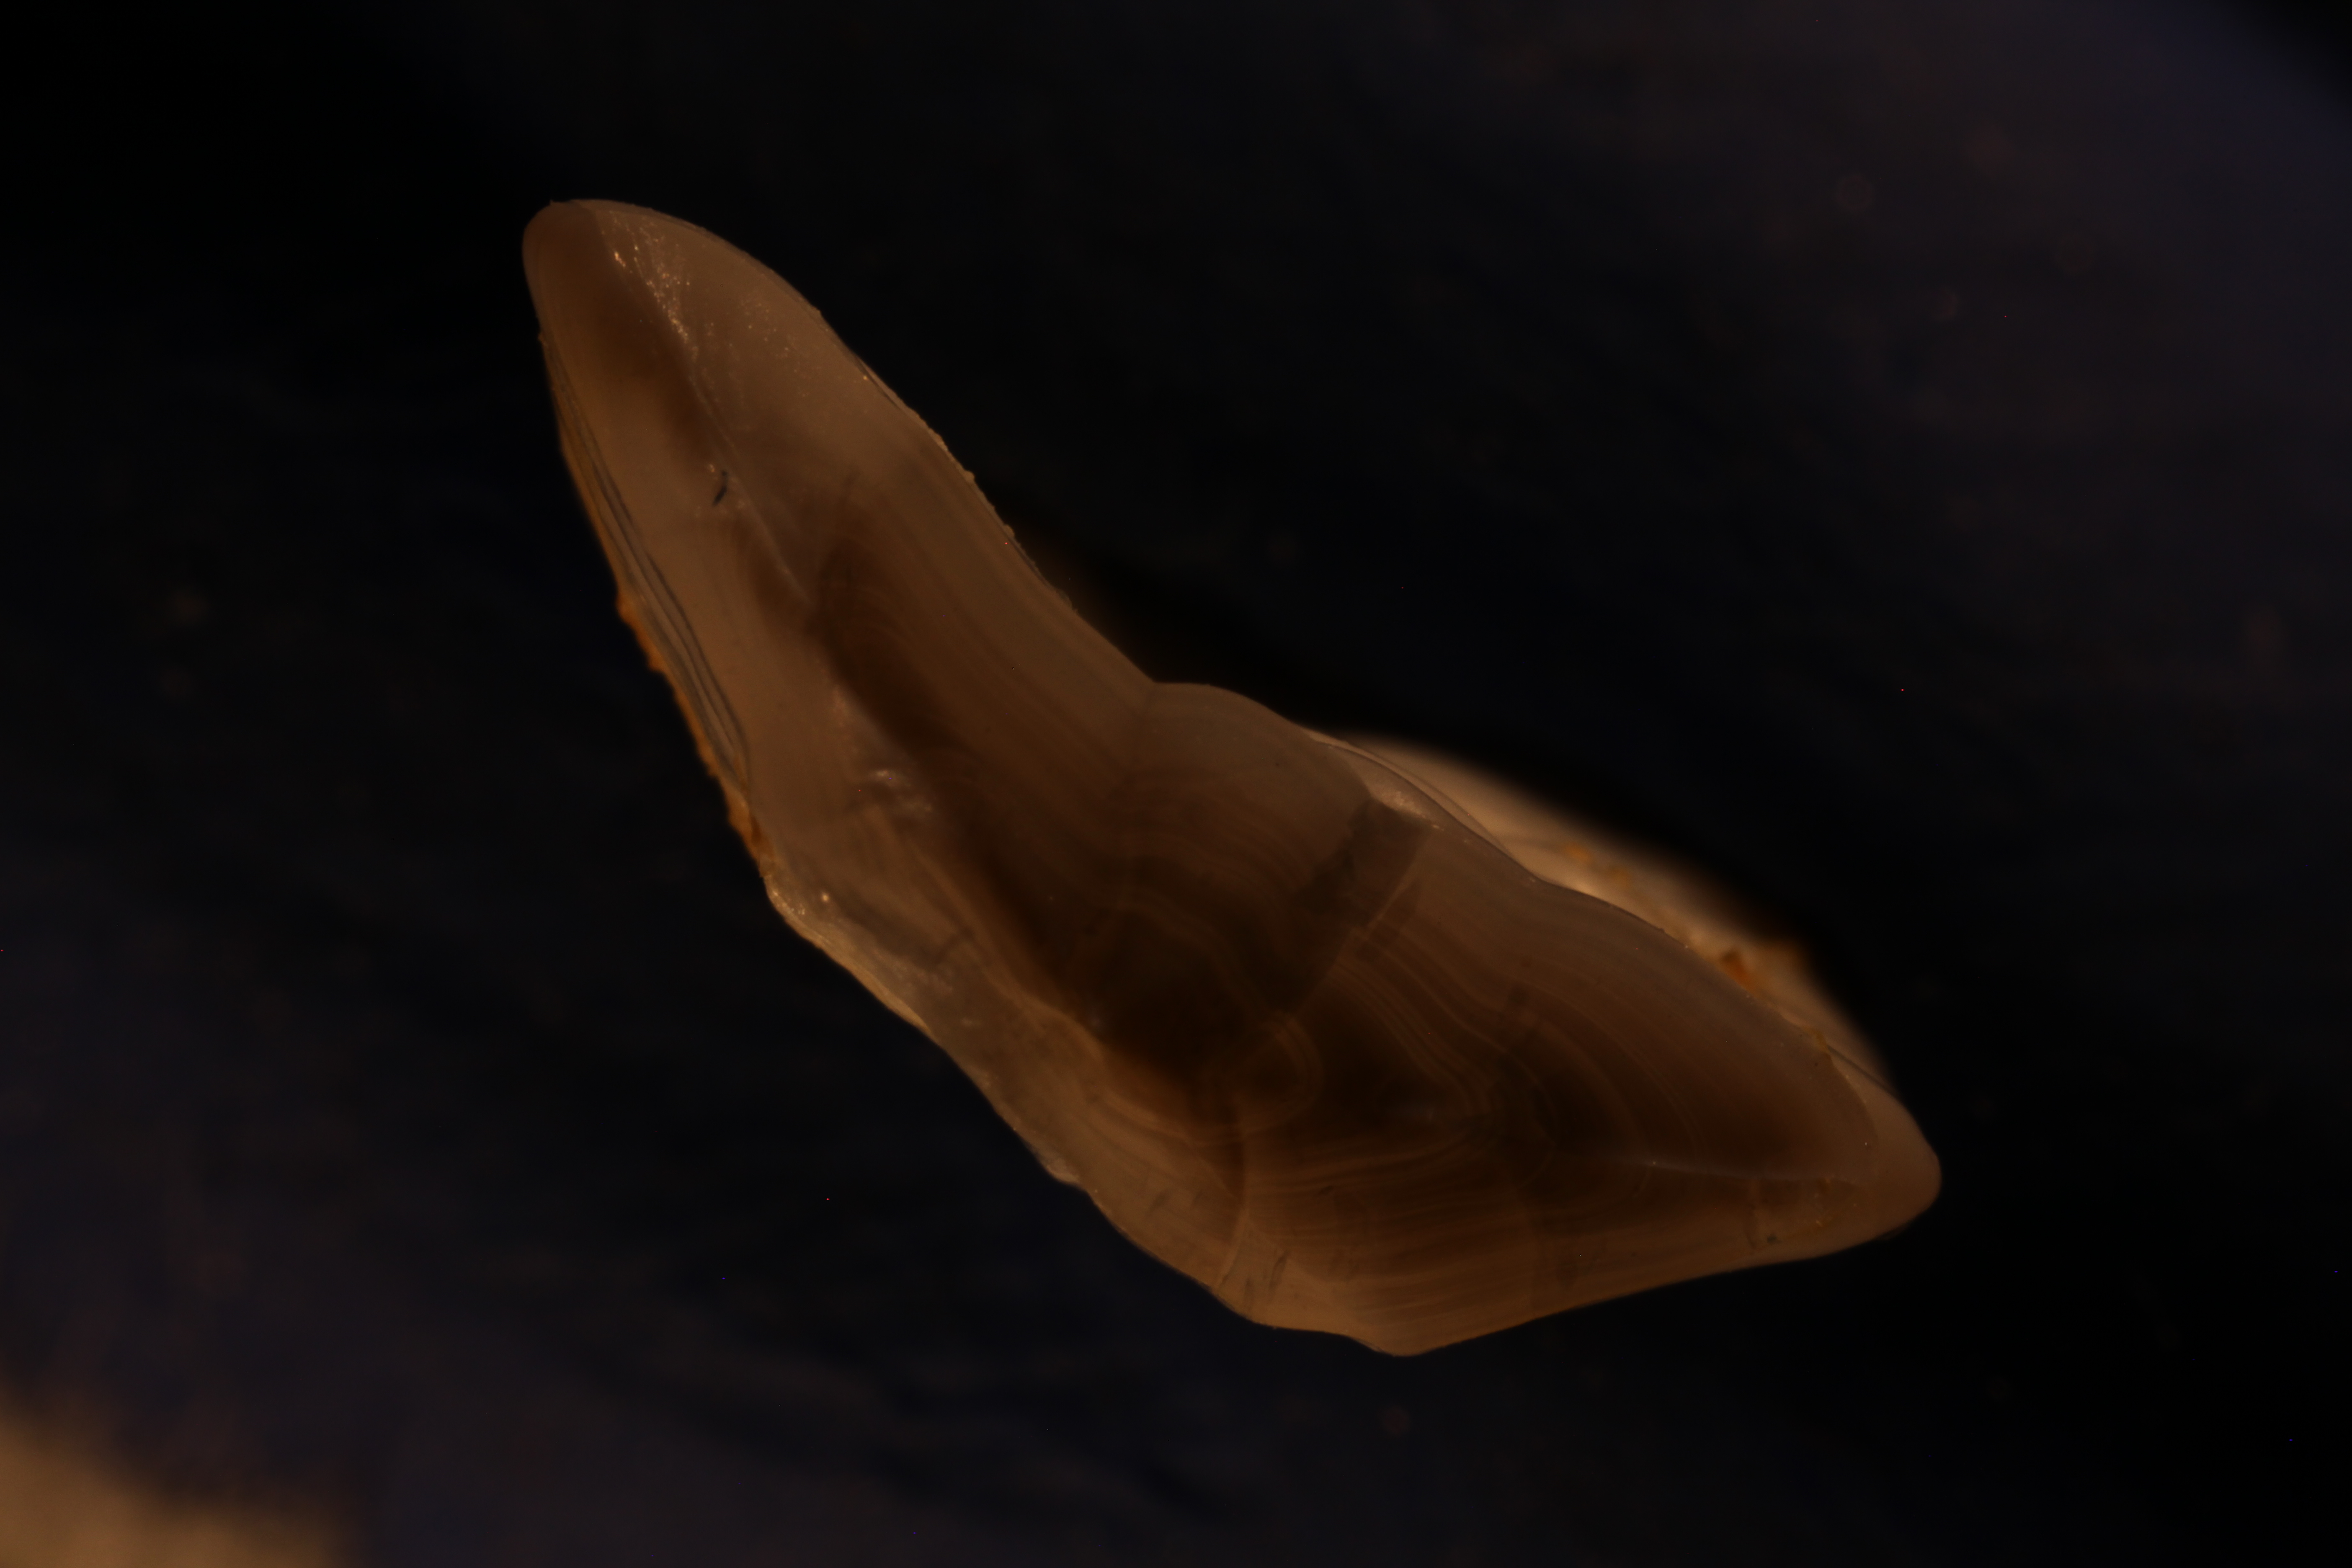
\includegraphics[scale=0.015]{otolith/IMG_0461_2016_70021.JPG}
  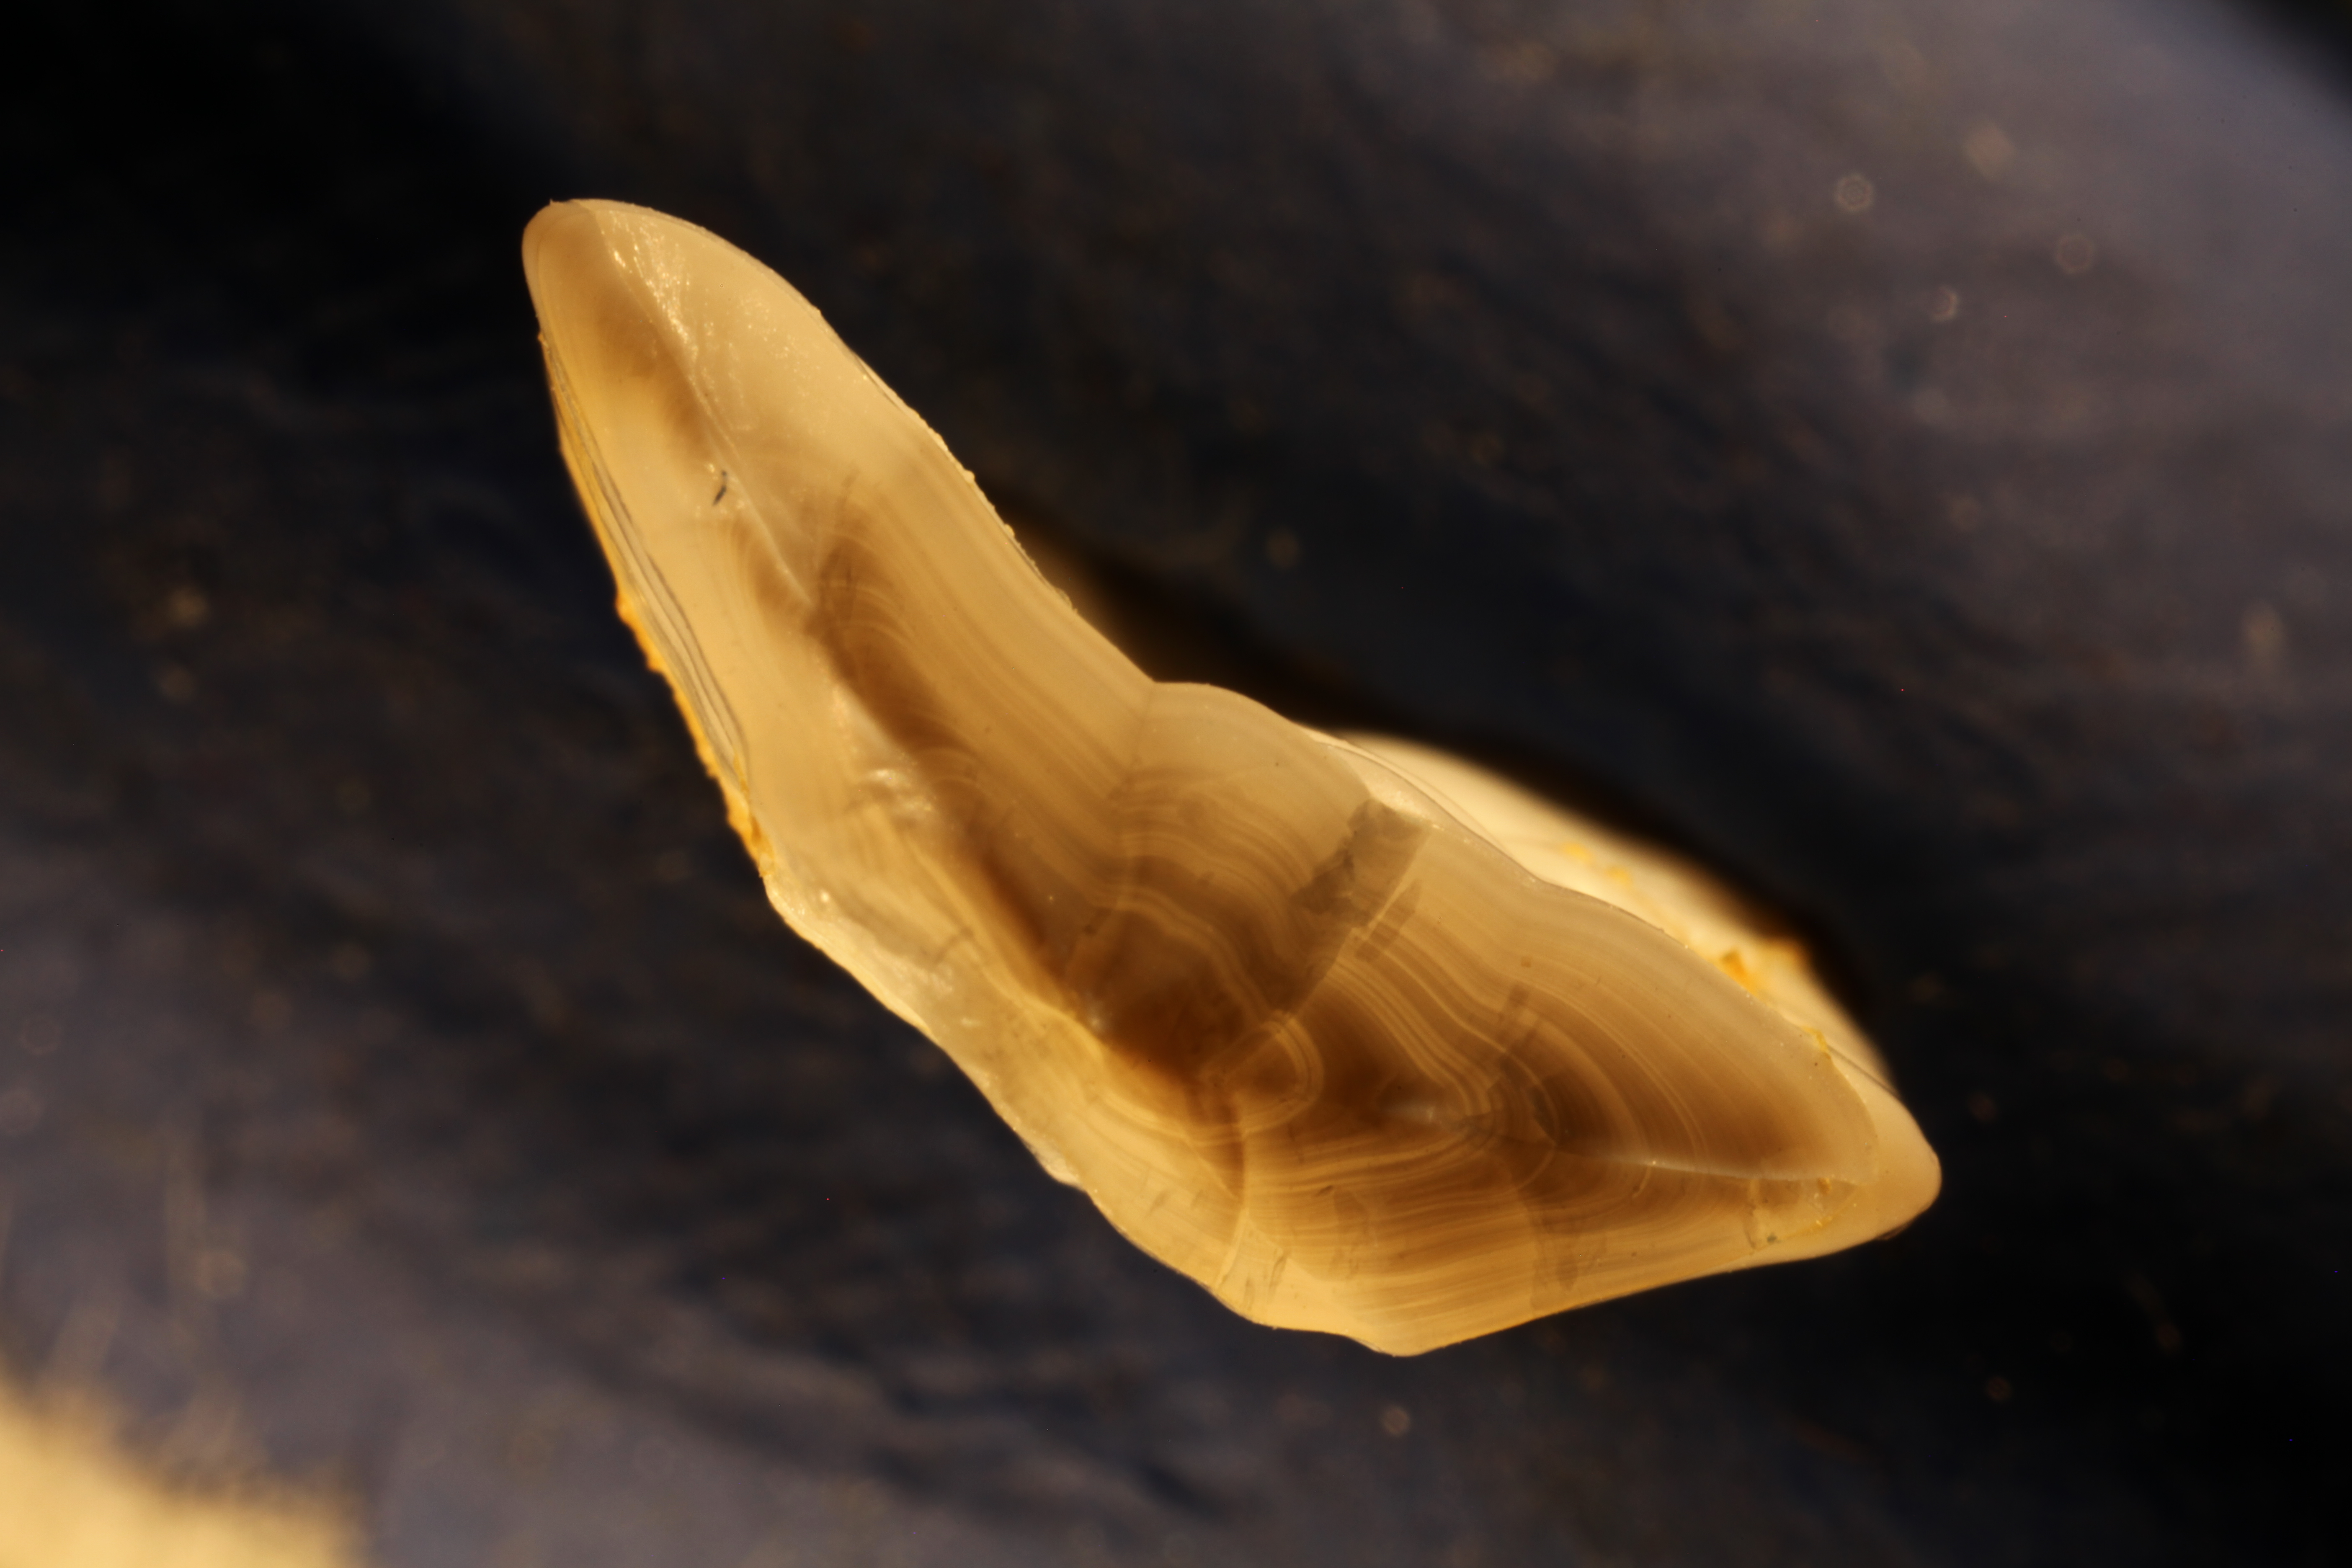
\includegraphics[scale=0.015]{otolith/IMG_0462_2016_70021.JPG}
  
  \label{marker1}
\end{figure}

The images is of size 3744 x 5616 which are re-scaled for training to between 384x384 to 512x512. The image light exposure varies depending on light condition outside, and are stored in the property 'ExposureTime' of the JPG file. Typically the exposure order is middle, dark, or light then a rotation of 180 degrees, and then middle, light, dark again. But the order might change, and
the given order is recovered by reading the metadata property of the jpeg and sorting the exposure time.

The otoliths are prepared for imaging by breaking them.
The process also involves a camera setup, a folder structure referencing 
age, survey and station number, lighting setup, mounting of camera, and 
finally camera capture. More information about this process
can be found in \Mycite{codOtolithsMyers}


\begin{figure}[h!]
  \centering
  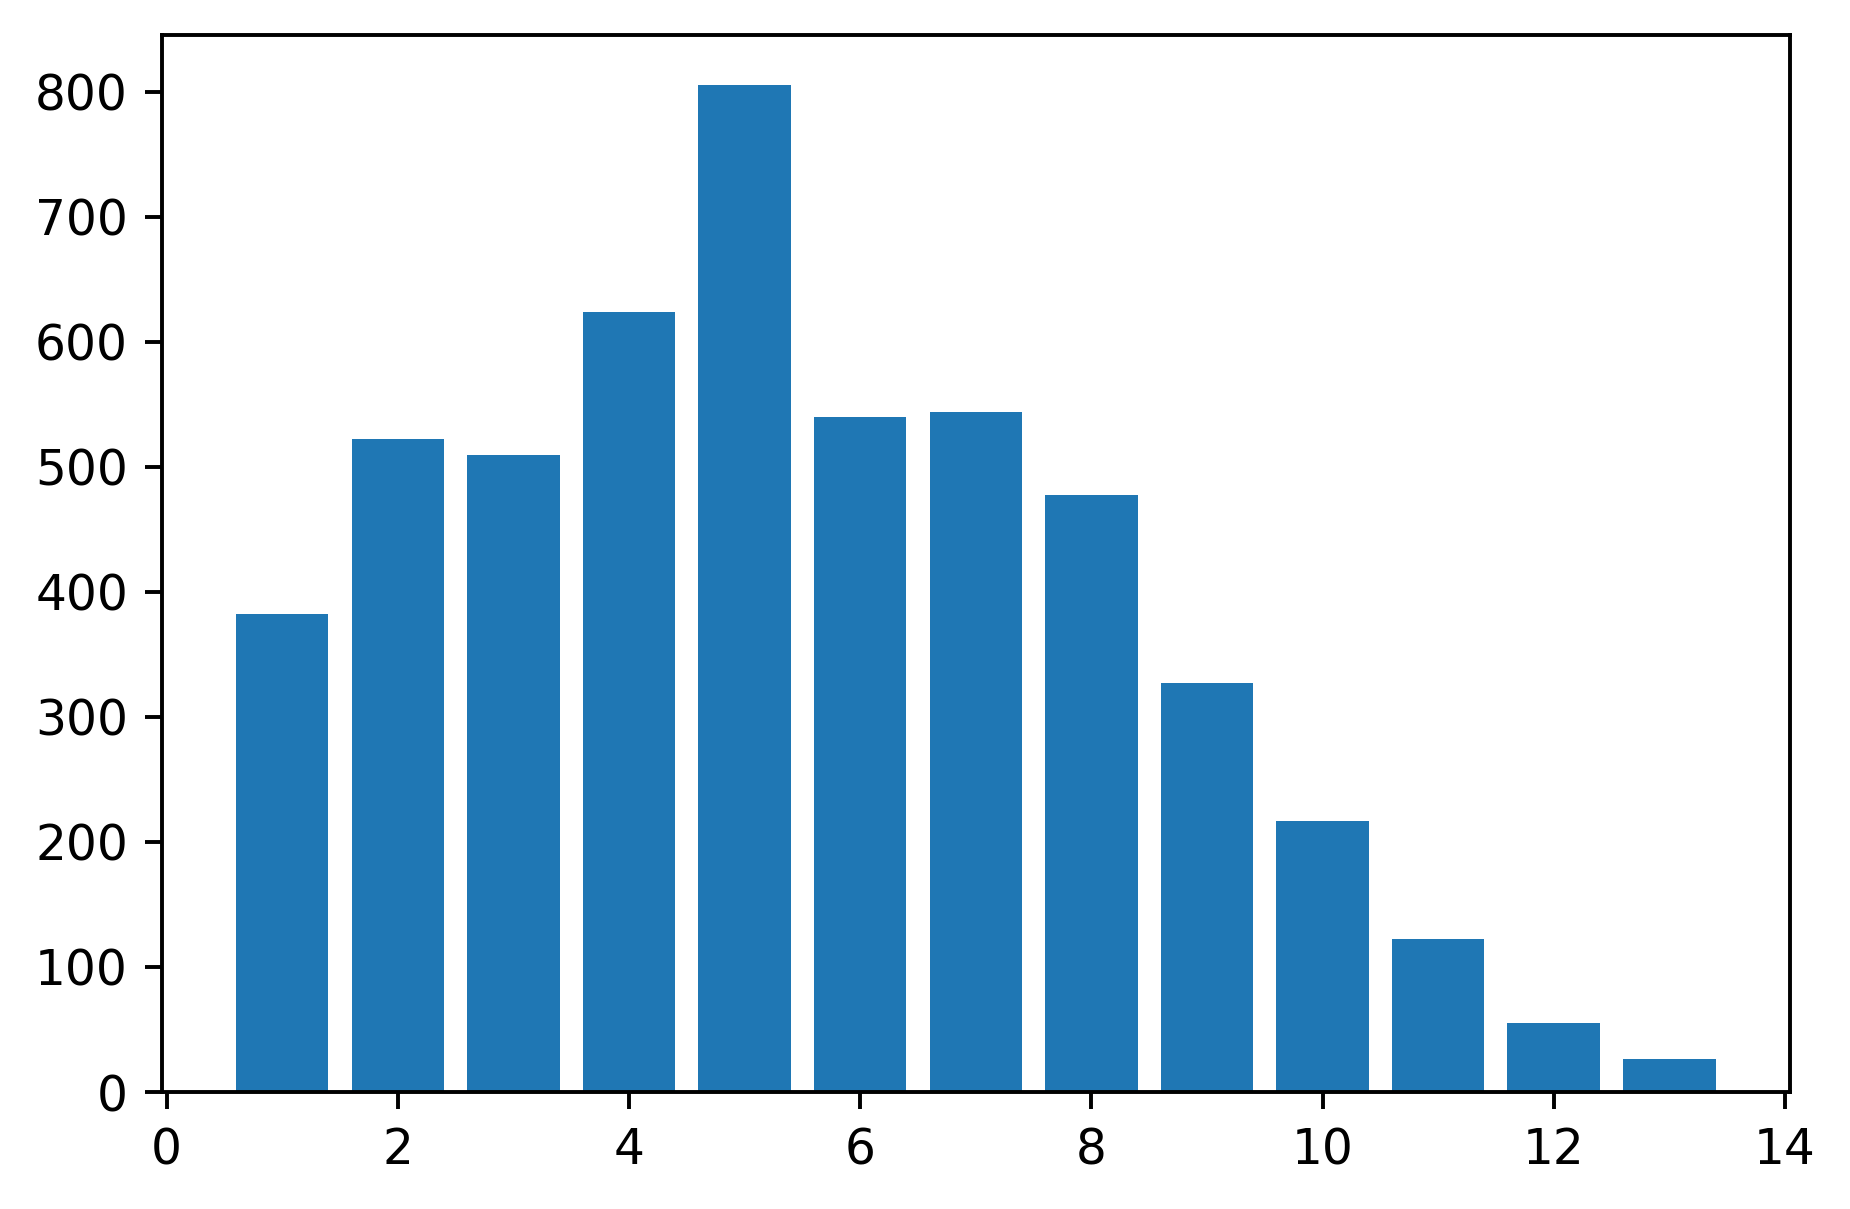
\includegraphics[scale=0.60]{distribution/age_distribution.png}
  \caption{Age distribution of all 5150 images}
\end{figure}

\begin{figure}[h!]
  \centering
  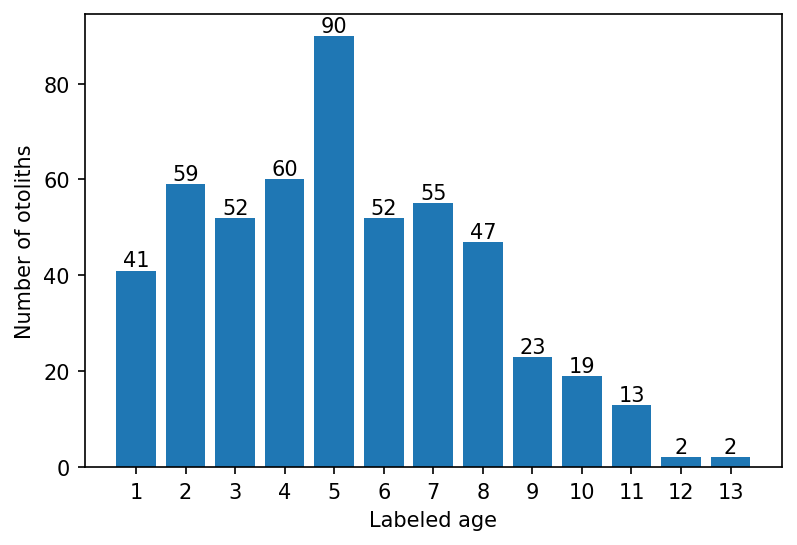
\includegraphics[scale=0.60]{distribution/age_distribution_test.png}
  \caption{Age distribution of 515 images from the test set}
\end{figure}

\subsection*{Preprocessing and augmentation}

To create a large data set with millions of images needed to evaluate the models, we use image augmentation. Image augmentation has made it possible to do deep CNN training on smaller data sets \citep{krizhevsky2012imagenet}. By using this technique it is possible to create millions of training images.

The augmentation methods that we use are rotation by 0 to 360 degrees, and reflection by the vertical (or horizontal) axis. This can be done without loss of information. Also the age reading is agnostic to orientation.

No other augmentation techniques was used like  cropping, shifting or shearing as it can result in loss of age structure information.

The augmented data set can produce 360*2*5150 = 3.708.000 possible images.
Depending on the augmentation factor and the number of images in a training cycle, the model will likely never see the same image twice.
% \citep{boureau2010theoretical} 

The data has been split into train and test-set with 10 \% test-set, 9 \% validation
and 81 \% training-set. Training has been done on the 90 \% of the data set, 4635 images, with 10-fold split producing 10 models. While predictions are made on the 515 images in the test set. The final prediction is
an ensemble prediction on the given model recorded as the expectation on predictions on the test set from the 10 models. 

\begin{figure}[h!]
  \caption{Otolith from 2013, read age: 6. With light exposure: medium, low, high, 
  and expectation per channel of the three exposures. }
  \centering
  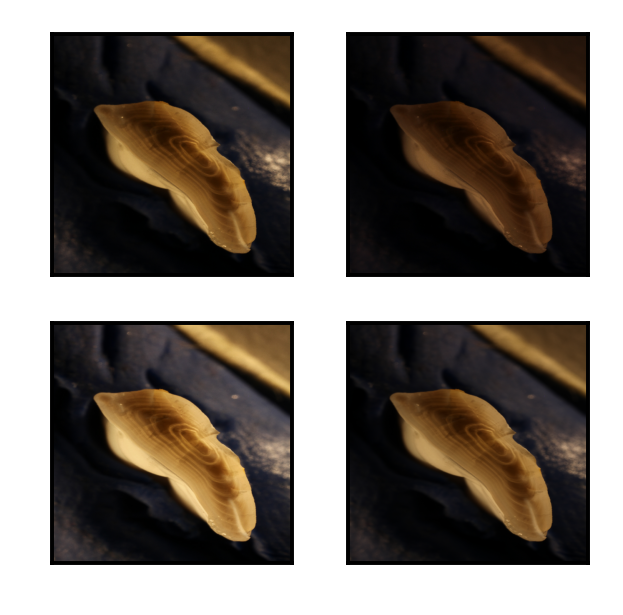
\includegraphics[scale=0.015]{otolith/2013_70174_Nr06_age09_IMG_0031_32_33.png}
  
  \label{marker1}
\end{figure}

\subsection*{Convolutional neural network}

There are two families of models used, EfficientNet B4-B6 \citep{EfficientNet}   from Tensorflow \citep{abadi2016tensorflow} with a Keras  \citep{keras} implementation plus weights, and a PyTorch \citep{PyTorch}  implementation of EfficientNet V2 medium, Large 
and Xtra-Large \citep{EfficientNetV2} implementation with weights from Timm\citep{Timm}. Weights are ImageNet \citep{imagenet} weights, which is another prerequisite when working with small data sets, in addition to augmentation. The image size varies between 380 and 528 for EfficientNet Bx, and 384 for EfficientNetV2 size medium, large and xtra-large. While test-set size prediction has been done both on 384 and larger resolutions 480 and 512 as described in the paper. To investigate the image-taking protocol described in \citep{codImageProtocol} we have is also training on 9-channel images. Three images are stacked to produce a 9-channel. Using Timm\citep{Timm} the imagenet weights are duplicated on the input layer to accommodate 9 channels. The 3 images used are of dark, medium and light exposure of the first orientation.

EfficientNetV2 has been modified sligtly because the objective is regression as opposed to classification. The output layer of EfficientNetV2 becomes input to a Multi-Layer Perceptron (MLP) of 256 and 32 layers and then to a linear activation function which is the predicted age. More specifically; the 1280 layers output from EfficientNetV2 is input to 256 layer-MLP, then a leakyRelu \citep{leakyRelu} then 32 layer-MLP, another leakyRelu, then a linear activation function is the output. This outperformed a linear activation on the 1280 layers from EfficientNetV2, likely because we are doing a regression.

We train and tune EfficientNet B4, B5, B6 \citep{2015arXiv151200567S}, EfficienetNetV2 m, l \citep{szegedy2015going}, and xl. 
The test results from top models are ensembled to produce the final prediction.

Hyper-parameter tuning is an important step when working with a new dataset and architecture. Some hyper-parameters
that as been tuned are batch size, learning rate, k-fold size, weight decay, step size, number of epochs, early stopping, and
patience. To keep track of all these parameters, a config.json file has been written for each model trained, and 
the exact configuration can be found the the results section of the github page of this project
(https://github.com/emoen/Deep-learning-for-regression-of-cod-otoliths)


\subsection*{Ensemble of ensembles}

As previously mentioned, the results recorded pr model is an ensemble of 10 models trained on 10-fold split of the
training data set. Typically the ensemble prediction is better than any single fold prediction. 
This result can be improved further by taking ensemble predictions of multiple models as prediction on the test set.
We look at all ensembles from tuple predictions consisting of 2 models, which produces an ensemble of 20 models,
to ensemble of all models which produces an ensemble consisting of 210 models. 
By choosing the best model we are over fitting to the test-set, but 
selecting a subset of the best of these ensembles should produce a candidate ensemble
of ensemble which will produce the best prediction on a test-set holdout set.

\subsection*{Evaluation metric}

The primary metric used for learning in the model is mean squared error (MSE)
defined as $  ( \hat{y} - y)^{2} $ where \hat{y} is the CNN prediction and y is the read age.
MSE produces a real number, while the prediction is a positive integer,
which is produced by rounding to nearest integer. 
The integer is used to measure accuracy. To reach human level accuracy
a score of 85\% or higher is required \citep{ref_needed}.

\section*{Results}

We have conducted a series of experiments on the EfficientNet family of CNNs, 
with different hyper-parameters and on images withlight exposures 
from the set light, medium, dark.
Training has been done on the 10-fold cross validation set which produced 10 models.
An ensemble of the best models produced the best accuracy score in table 3.1

\begin{center}
\begin{table}[hbt!]
\caption{Accuracy on: light exposure/CNN architecture}
\begin{tabular}{ |l|c|c|c|c|c|c| }

\hline
lighting/CNN in acc & B4 & B5 & B6 & Medium & Large +MLP & Xtra Large \\ \hline
min & 72.8 & 74.4 & 73.4 & 67.0* & - & - \\ 
medium & - & - & - & 64.3* & 71.8 & - \\ 
max & - & - & - & 65.8 & - & - \\ 
9 channels & - & - & - & - & 71.7 & - \\ 
\hline
\end{tabular}
\end{table}
\end{center}

\begin{center}
\begin{table}[hbt!]
\caption{MSE on: light exposure/CNN architecture}
\begin{tabular}{ |l|c|c|c|c|c|c| }

\hline
lighting/CNN in acc & B4 & B5 & B6 & Medium+MLP & Large+MLP & Xtra Large \\ \hline
min & .277 & .277 & .272 & .331* & - & - \\ 
medium & - & - & - & .292 & .280 & - \\ 
max & - & - & - & .381 & - & - \\ 
9 channels & - & - & - & - & .281 & - \\ 
\hline
\end{tabular}
\end{table}
\end{center}


\begin{figure}[h!]
  \centering
  \begin{minipage}[b]{0.49\textwidth}
  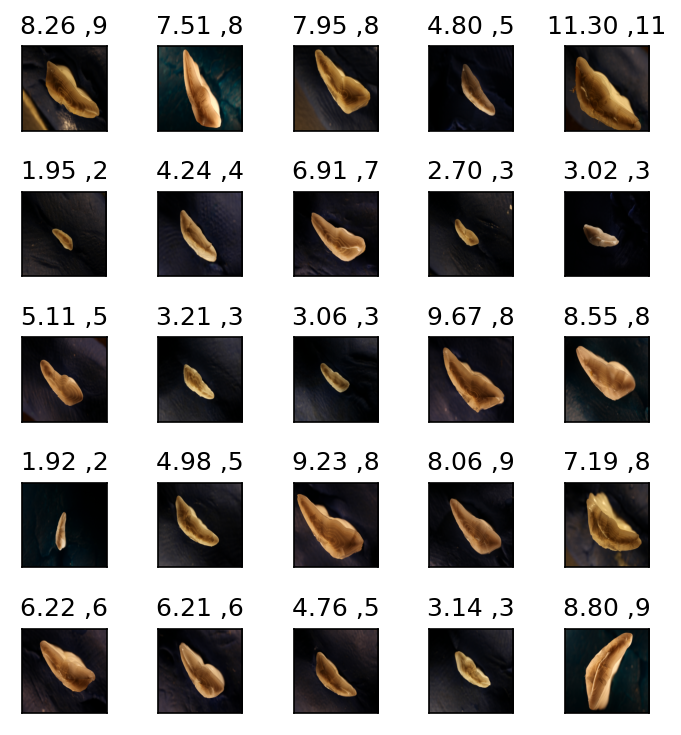
\includegraphics[scale=0.5]{results/fold_prediction_V2_m.png}
    \caption{Sample of 25 predictions on a fold of training on EfficientNetV2 medium}
   \label{marker5}
  \end{minipage}
  \hfill
\end{figure}

The models predicted can be viewed in a box plot

\begin{figure}[h!]
  \centering
  \begin{minipage}[b]{0.49\textwidth}
  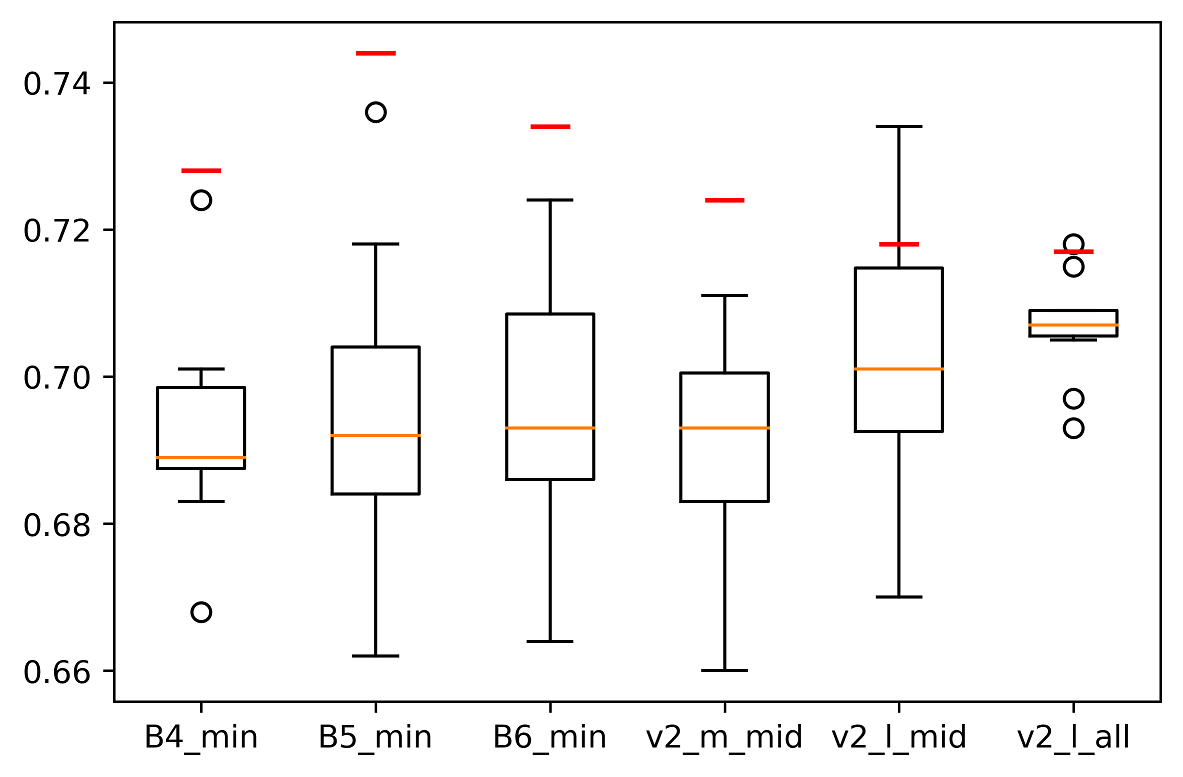
\includegraphics[scale=0.2]{results/box_plot_models_acc.png}
    \caption{Accuracy score of 5 models and red line is ensemble prediction accuracy}
   \label{marker5}
  \end{minipage}
  \hfill
\end{figure}

\begin{figure}[h!]
  \centering
  \begin{minipage}[b]{0.49\textwidth}
  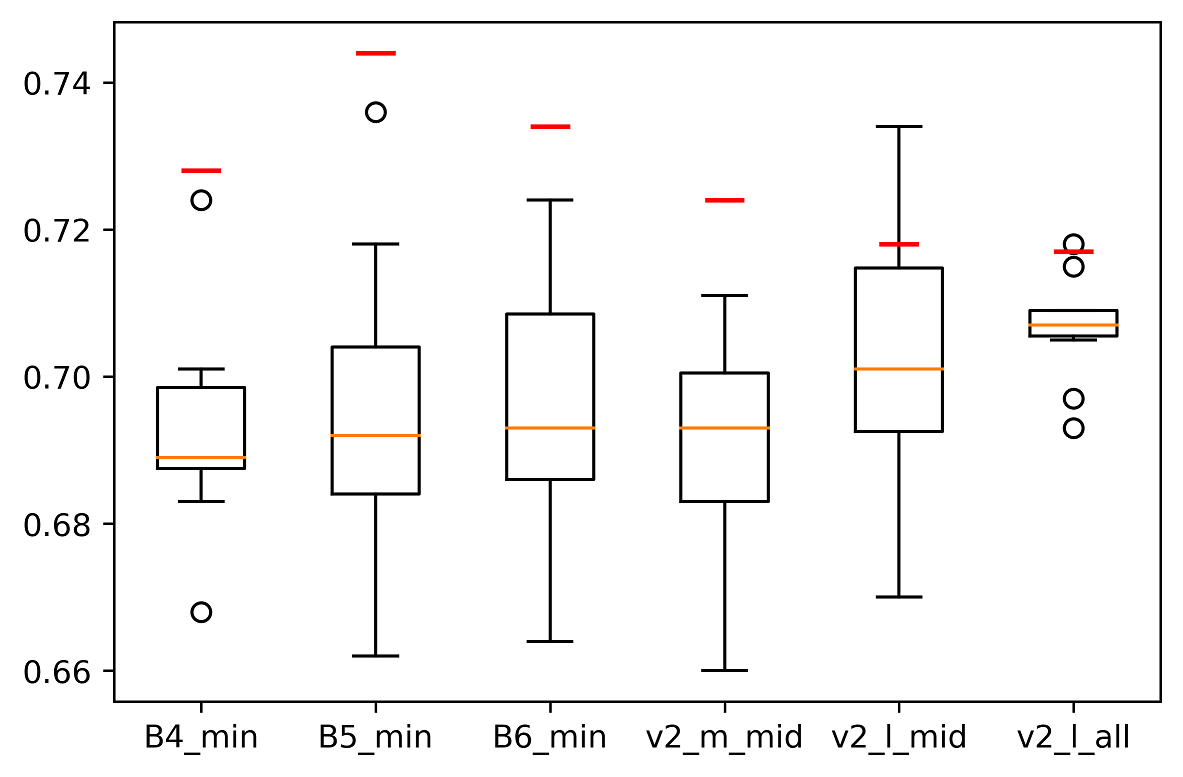
\includegraphics[scale=0.2]{results/box_plot_models_acc.png}
    \caption{MSE score of 5 models and red line is ensemble prediction MSE}
   \label{marker5}
  \end{minipage}
  \hfill
\end{figure}


\subsection*{Ensemble of ensembles}

\subsection*{Outliers}

Looking at figure (x) we can see that the model under predicts the age of older otoliths. This pattern is especially observable for individuals read as 15 years and older. The oldest predication is 18 years while the test set contains individuals as old as 22 years. To better understand the bias, figure \ref{marker5} shows the 4 largest outliers from the test set which come from two pairs

\begin{figure}[h!]
  \caption{The most common images miss predicted with more than 1.5 years}
  \centering
  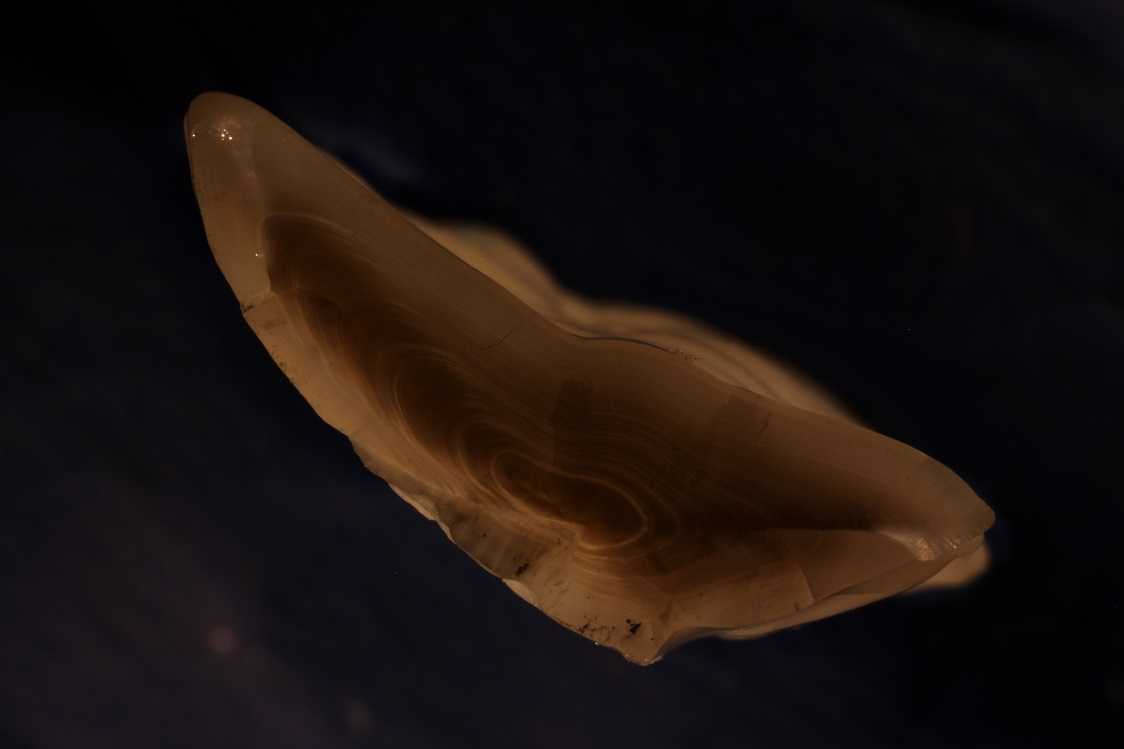
\includegraphics[scale=0.1]{outliers/IMG_0284_13.JPG}
  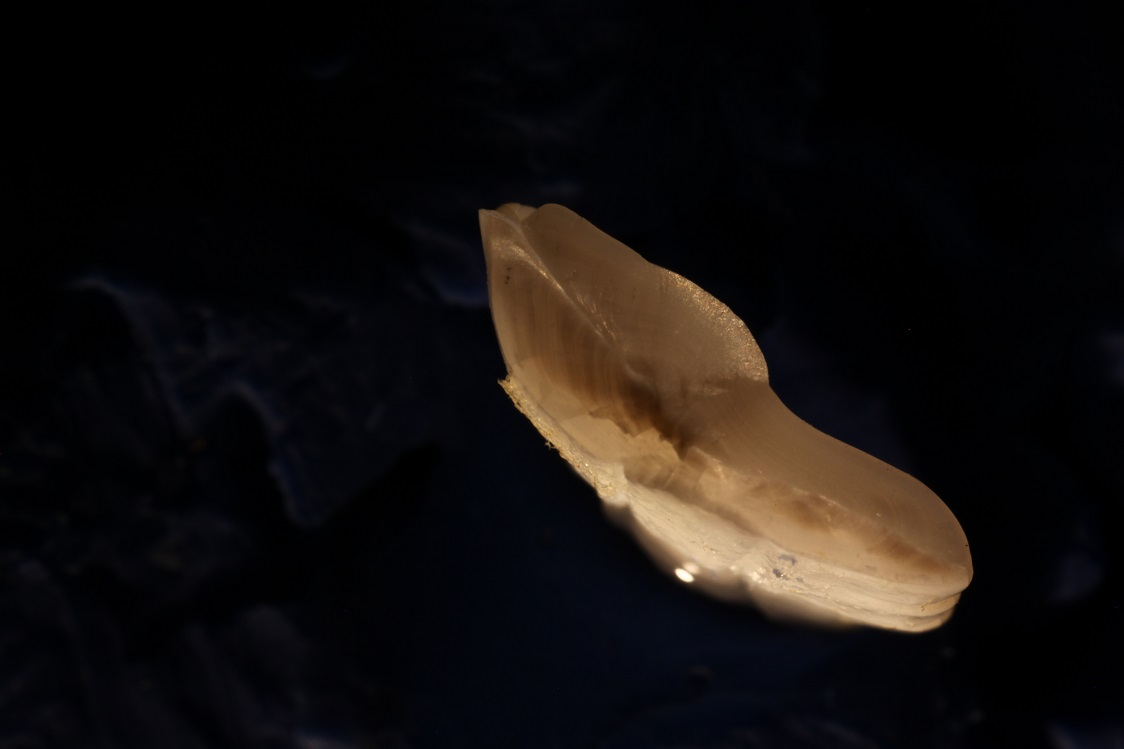
\includegraphics[scale=0.1]{outliers/IMG_0230_71.JPG}
  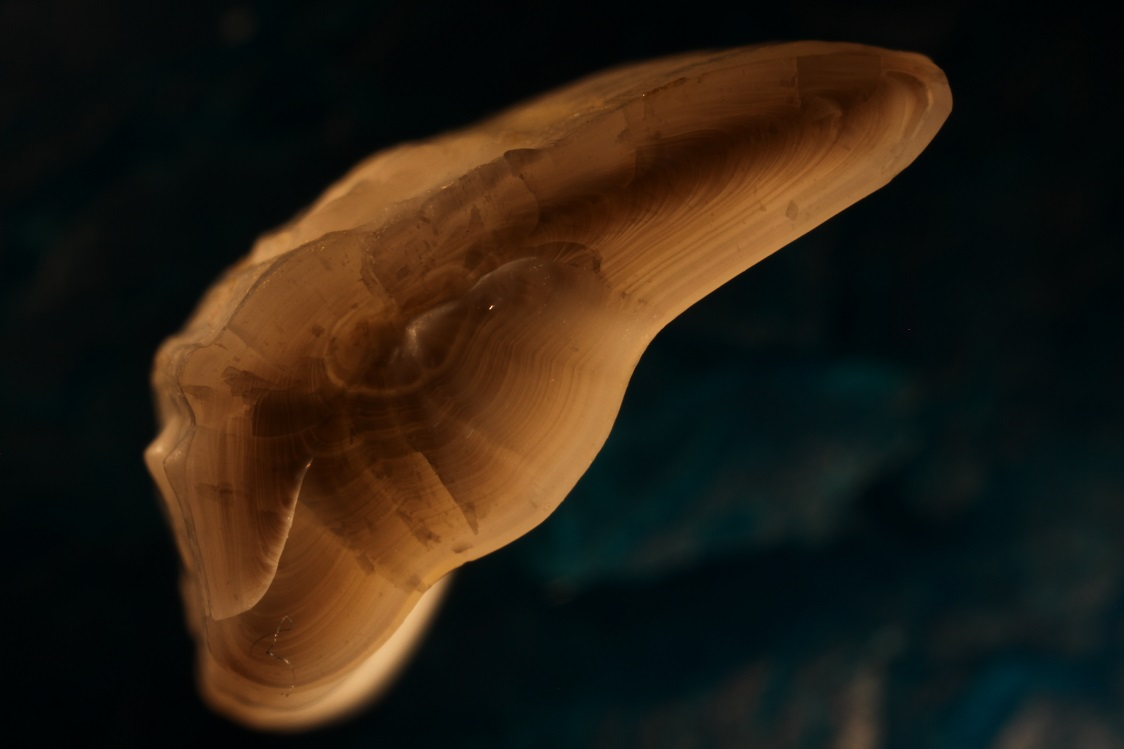
\includegraphics[scale=0.1]{outliers/IMG_0104_270.JPG}
  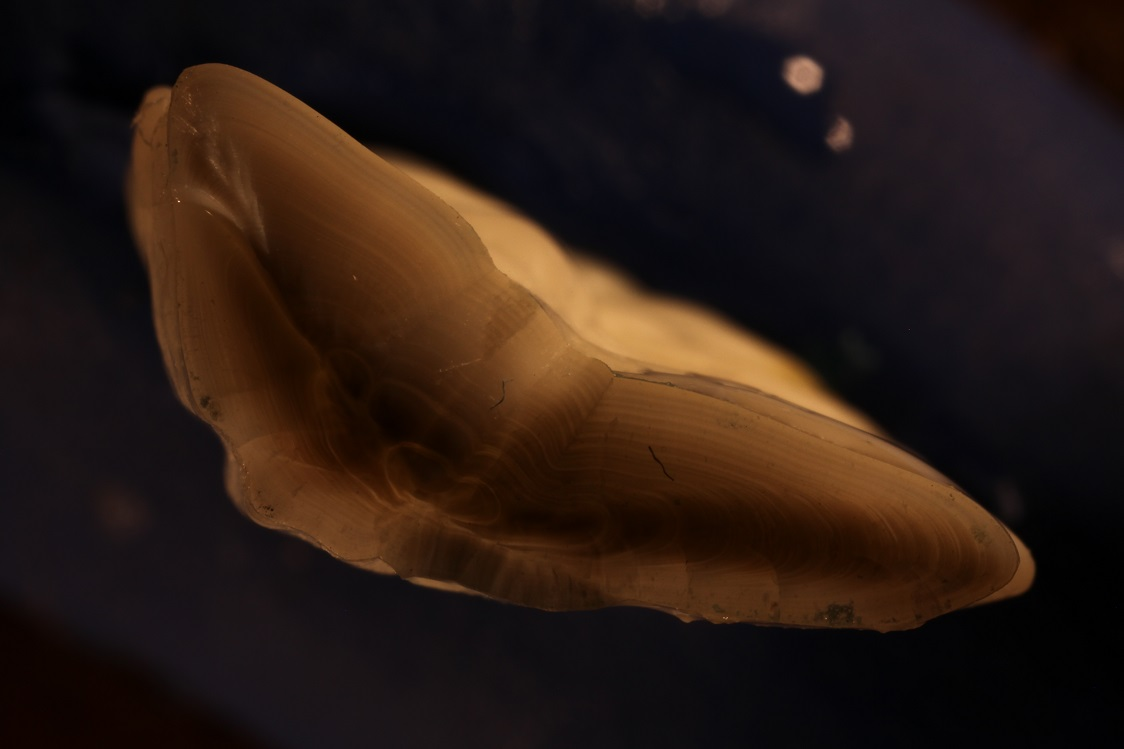
\includegraphics[scale=0.1]{outliers/IMG_0044_342.JPG}
  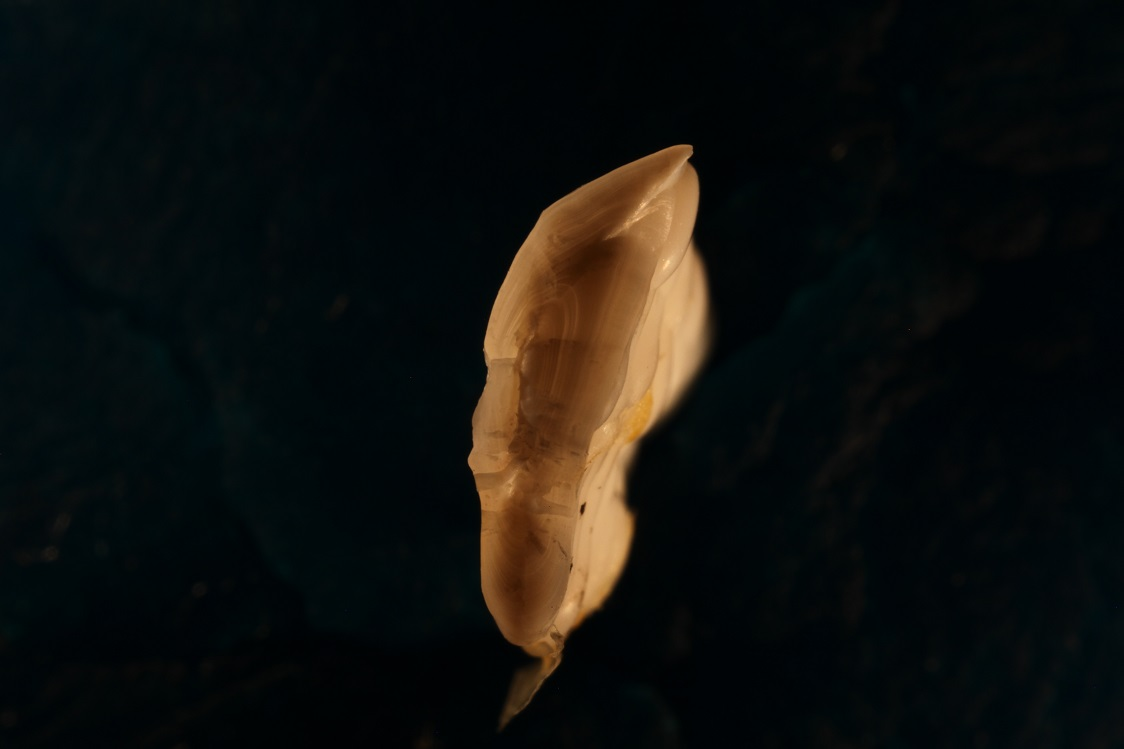
\includegraphics[scale=0.1]{outliers/IMG_0086_360.JPG}
  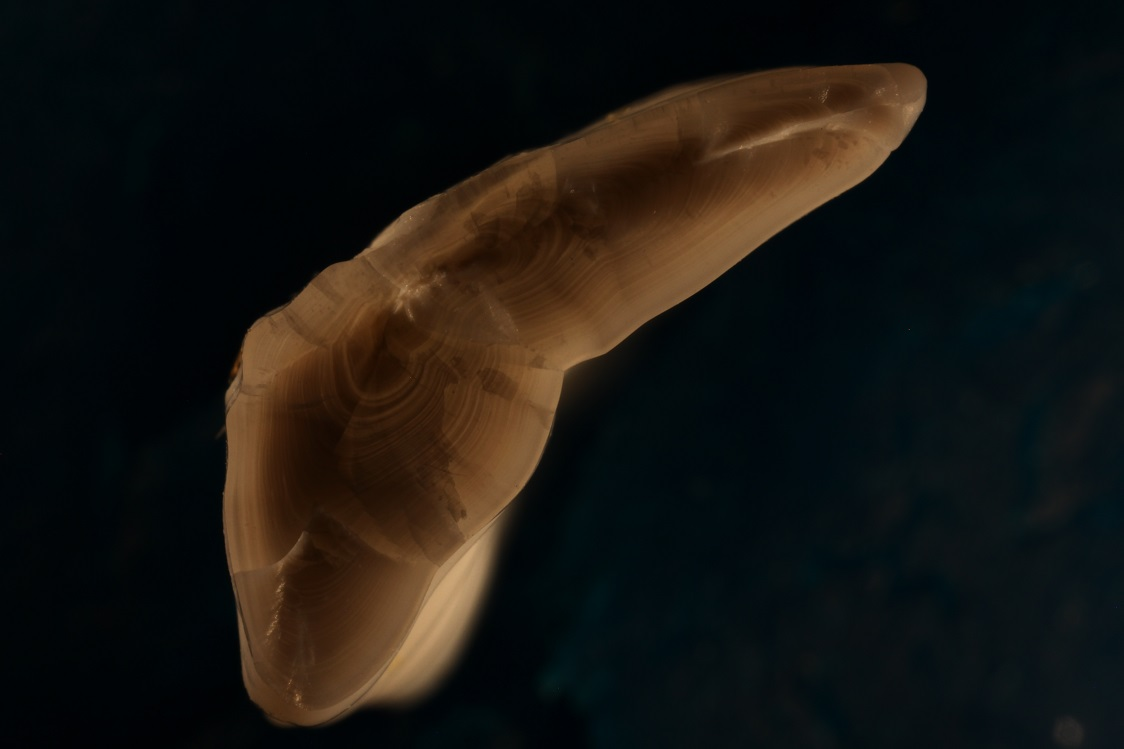
\includegraphics[scale=0.1]{outliers/IMG_0122_369.JPG}
  \label{marker7}
\end{figure}

Figure \ref{marker7} are the most commonly mis-classified images 
with greatest magnitude of error.


\section*{Discussion}

\subsection*{Convolutional neural network}

\section*{References}

\bibliographystyle{apalike}
\bibliography{references}

\end{document}
